%%%%%%%%%%%%%%%%%%%%%%%%%%%%%%%%%%%%%%%%%%%%%%%%%%%
\begin{frame}
  \begin{center}
    {\Large Keras}
  \end{center}
\end{frame}
%
%
%%%%%%%%%%%%%%%%%%%%%%%%%%%%%%%%%%%%%%%%%%%%%%%%%%%%
%\begin{frame}[fragile] \frametitle{}
%
%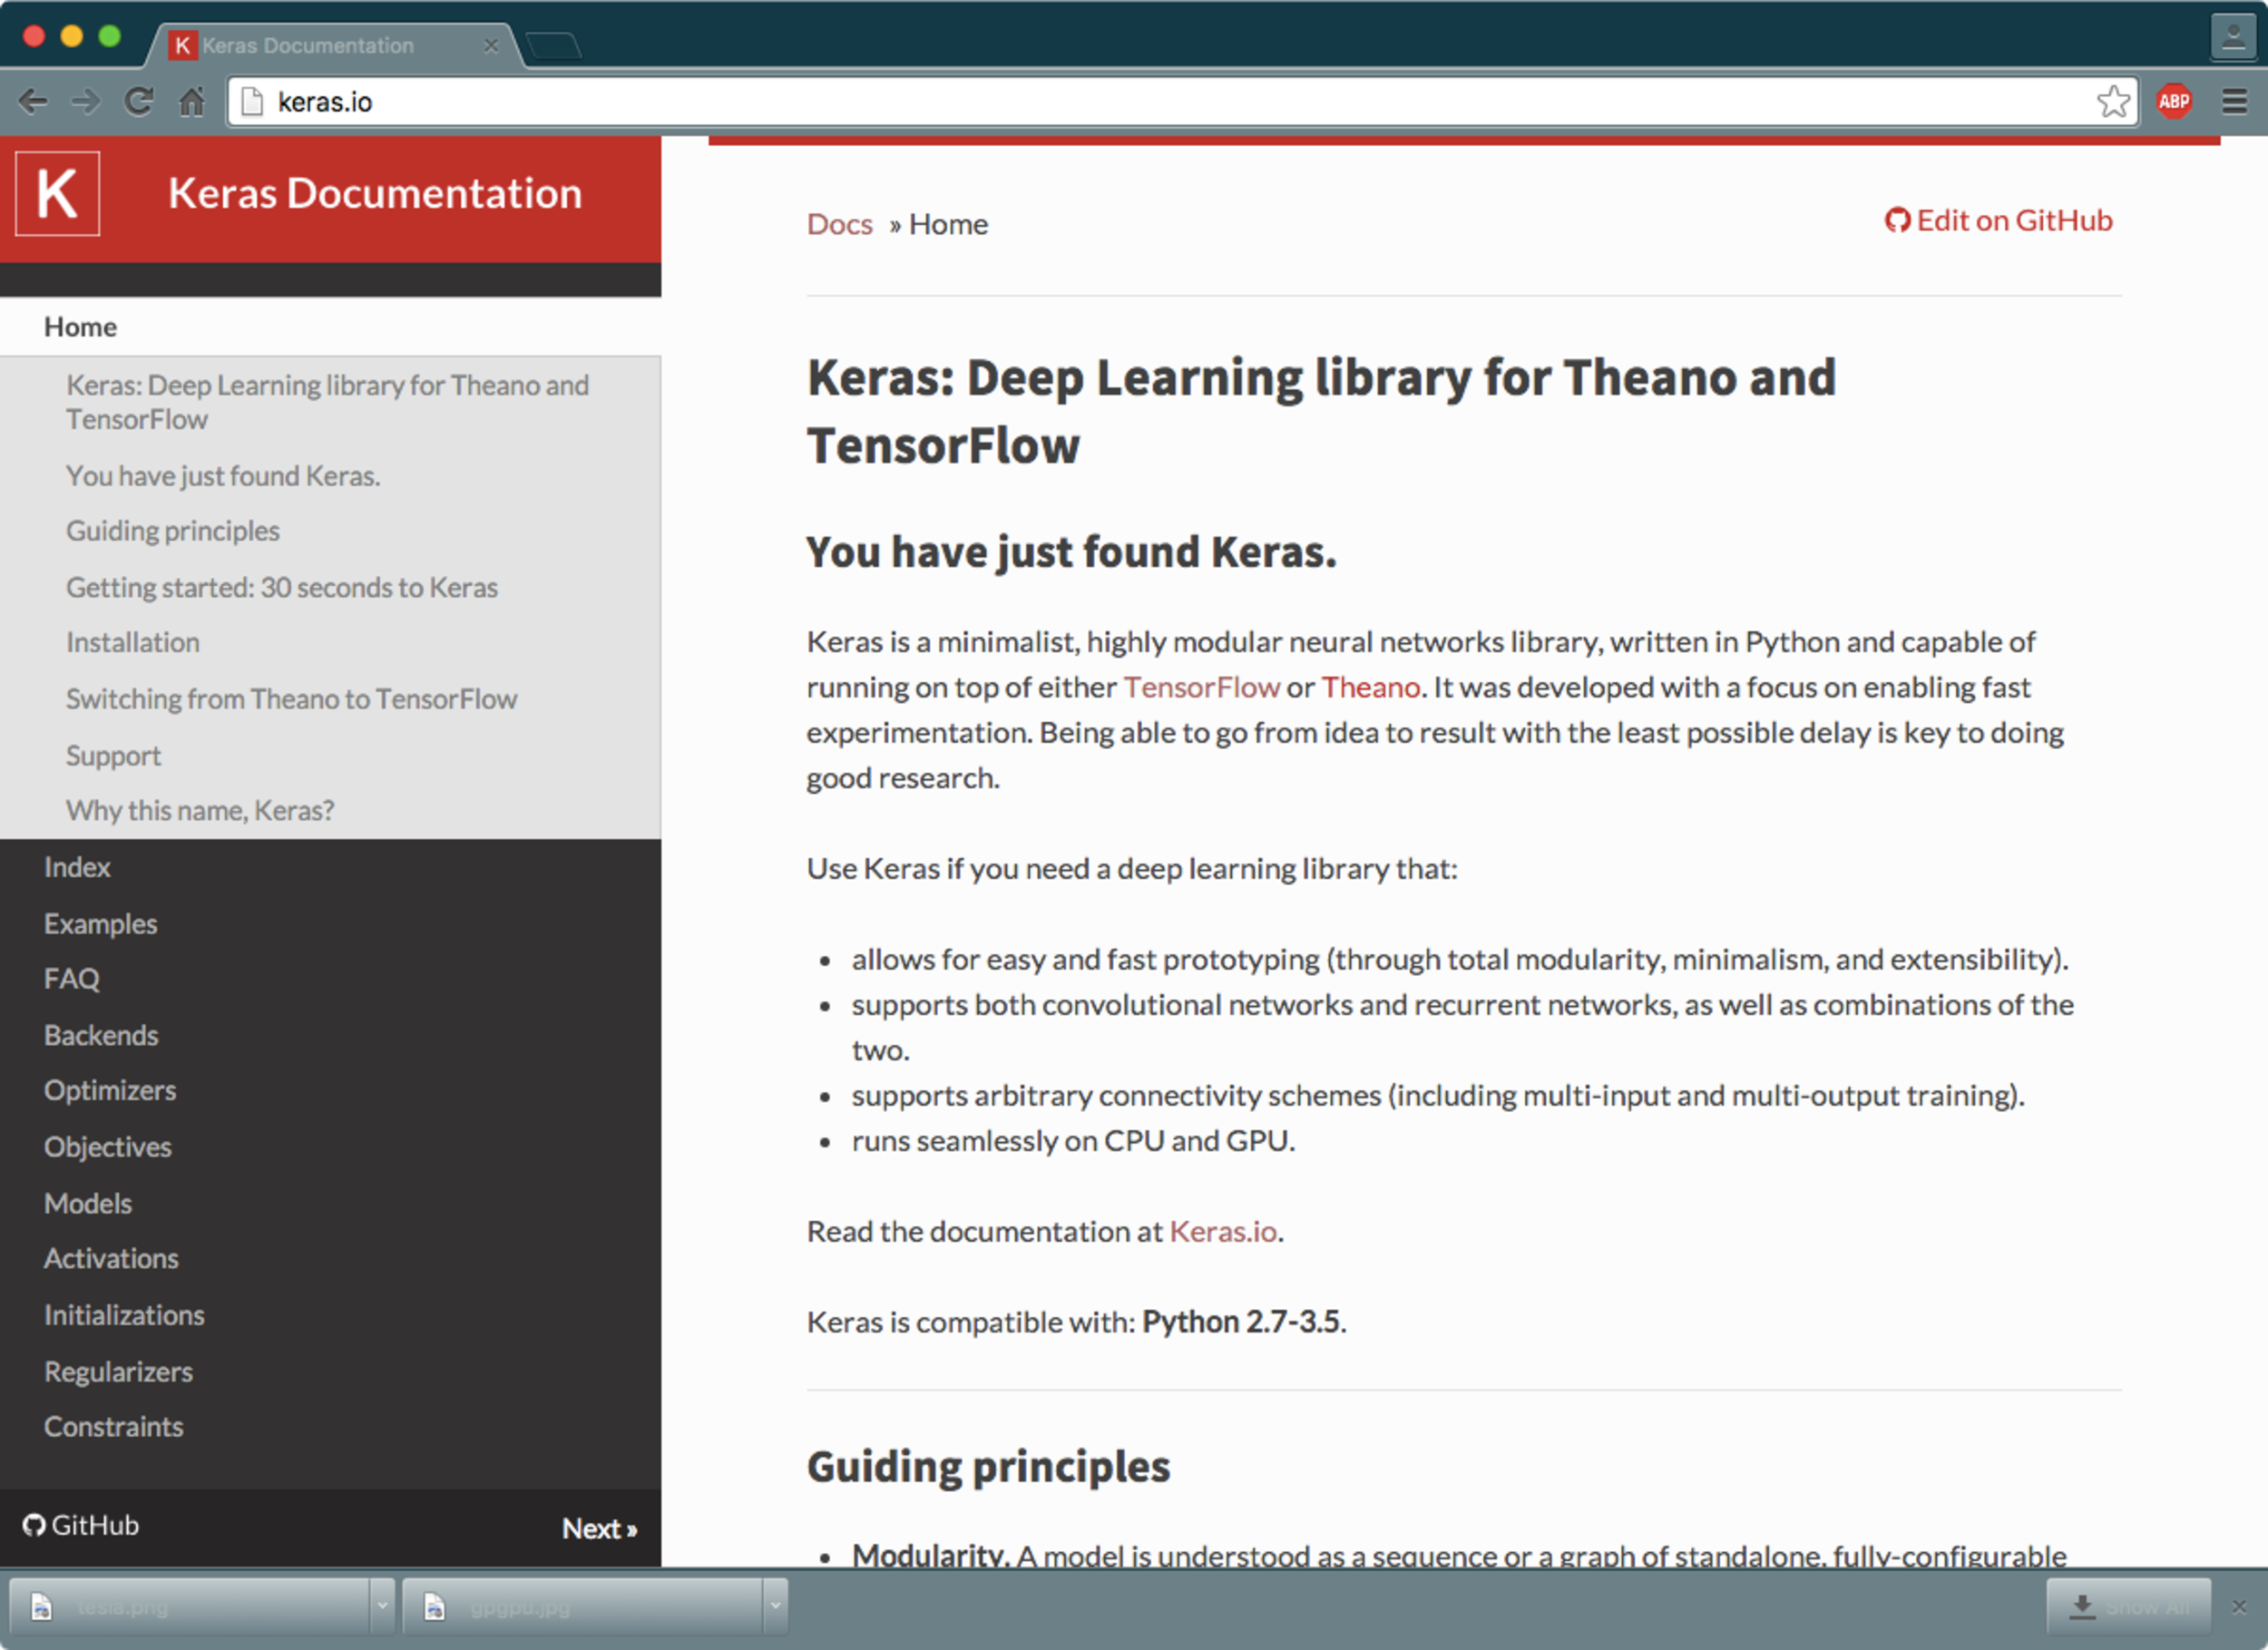
\includegraphics[width=\linewidth]{keras.pdf}
%
%\end{frame}
%
%%%%%%%%%%%%%%%%%%%%%%%%%%%%%%%%%%%%%%%%%%%%%%%%%%%%
%\begin{frame}[fragile] \frametitle{}
%\begin{itemize}
%\item For an input vector $x$ and a response $y$, we can view the network
%as simply being something like:
%\begin{align}
%z^1 &= W^1 a^0 + b^1 \\
%a^1 &= \sigma(z^1) \\
%z^2 &= W^2 a^1 + b^2 \\
%a^2 &= \sigma(z^2) \\
%z^3 &= W^3 a^2 + b^3 \\
%a^3 &= \sigma(z^3) \\
%\text{Cost} &= (y - a^3)^2
%\end{align}
%\item Each level can be described by a \textit{module}. 
%\item The $z$ layers
%are called linear layers, the $a$'s as sigmoid layers, and the last
%line is simply the cost function.
%\item The activation functions
%are now their own layers, which actually simplifies things mathematically.
%\end{itemize}
%\end{frame}
%
%%%%%%%%%%%%%%%%%%%%%%%%%%%%%%%%%%%%%%%%%%%%%%%%%%%%
%\begin{frame}[fragile] \frametitle{}
%
%Each type of module needs to be able to:
%\begin{itemize}
%\item take an input and return an output for the current tuning parameters
%\item calculate the matrix $\frac{\partial \text{output}_i}{\partial \text{input}_j}$
%\item calculate the set $\frac{\partial \text{output}_i}{\partial \text{parameters}_j}$
%\item store the tuning parameters
%\item update parameters from a minibatch
%\end{itemize}
%If all of these is readily implemented, one can simply chain together
%modules and have a built-in algorithm for learning from input data.
%
%\end{frame}
%
%%%%%%%%%%%%%%%%%%%%%%%%%%%%%%%%%%%%%%%%%%%%%%%%%%%%
%\begin{frame}[fragile] \frametitle{}
%
%An example, using the \textbf{keras} library, describes this
%well:
%\begin{lstlisting}
%model = Sequential()
%model.add(Dense(64, input_dim=20, init='uniform'))
%model.add(Activation('sigmoid'))
%model.add(Dropout(0.5))
%model.add(Dense(64, init='uniform'))
%model.add(Activation('sigmoid'))
%model.add(Dropout(0.5))
%model.add(Dense(10, init='uniform'))
%model.add(Activation('softmax'))
%\end{lstlisting}
%Where dense refers to a linear connected layer.
%
%\end{frame}

%%%%%%%%%%%%%%%%%%%%%%%%%%%%%%%%%%%%%%%%%%%%%%%%%%%
\begin{frame}
  \begin{center}
    {\Large Introduction}
	
	\tiny{(Ref: Deep Learning using Keras- alyosamah, Introduction to Keras - Francois Chollet)}
   
  \end{center}
\end{frame} 

%%%%%%%%%%%%%%%%%%%%%%%%%%%%%%%%%%%%%%%%%%%%%%%%%%%
\begin{frame}[fragile] \frametitle{What is Keras?}

\begin{itemize}
\item  Neural Network library written in python
\item  Design to be simple and straightforward
\item  Built on top of different deep learning 
libraries such as Tensorflow, Theano and 
CNTK
\end{itemize}

\begin{center}
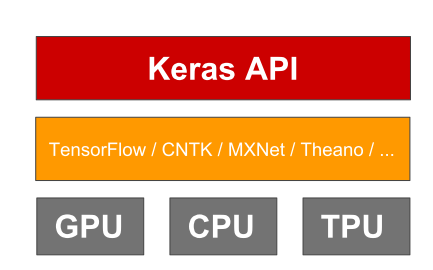
\includegraphics[width=0.5\linewidth,keepaspectratio]{kr16}
\end{center}

\end{frame}

%%%%%%%%%%%%%%%%%%%%%%%%%%%%%%%%%%%%%%%%%%%%%%%%%%%
\begin{frame}[fragile] \frametitle{Who makes Keras?}

\begin{center}

\includegraphics[width=\linewidth,keepaspectratio]{kr17}
\end{center}


\end{frame}

%%%%%%%%%%%%%%%%%%%%%%%%%%%%%%%%%%%%%%%%%%%%%%%%%%%
\begin{frame}[fragile] \frametitle{When to use Keras ?}

\begin{itemize}
\item  If you're a beginner 
and interested in 
quickly implementing 
your ideas:  Python + Keras: Super fast 
implementation, good 
extensibility
\item  If you want to do 
fundamental research 
in Deep Learning:  Python + Tensorflow or 
PyTorch: Excellent 
extensibility
\end{itemize}
\end{frame}



%%%%%%%%%%%%%%%%%%%%%%%%%%%%%%%%%%%%%%%%%%%%%%%%%%%
\begin{frame}[fragile] \frametitle{Keras is a trend}
\begin{center}
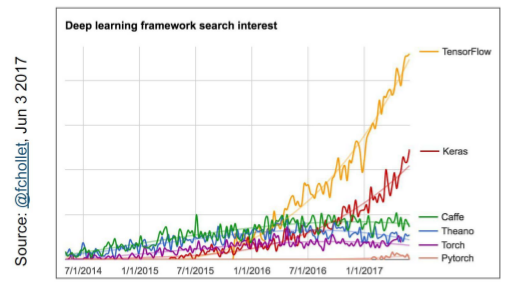
\includegraphics[width=\linewidth,keepaspectratio]{kr1}
\end{center}

\end{frame}

%%%%%%%%%%%%%%%%%%%%%%%%%%%%%%%%%%%%%%%%%%%%%%%%%%%
\begin{frame}[fragile] \frametitle{Keras developers}
\begin{center}
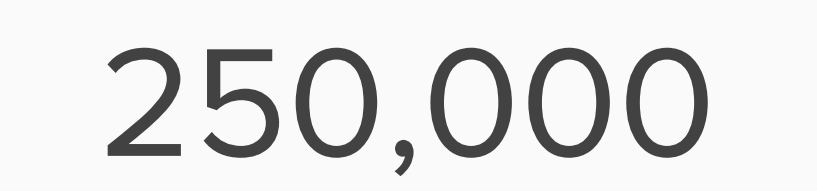
\includegraphics[width=\linewidth,keepaspectratio]{kr18}
\end{center}

\end{frame}

%%%%%%%%%%%%%%%%%%%%%%%%%%%%%%%%%%%%%%%%%%%%%%%%%%%
\begin{frame}[fragile] \frametitle{Research traction}
\begin{center}
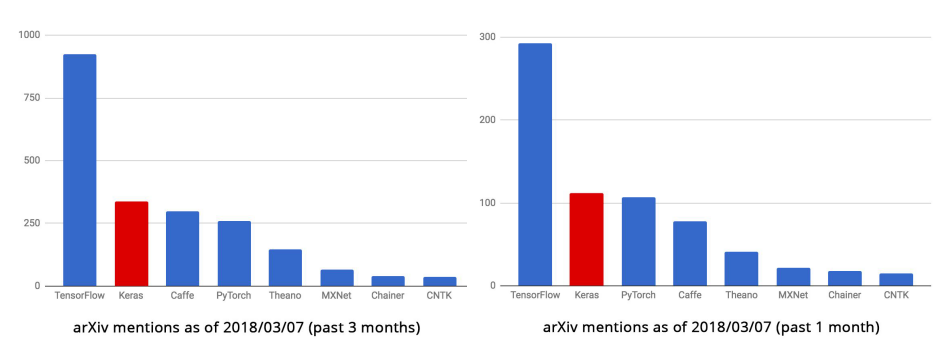
\includegraphics[width=\linewidth,keepaspectratio]{kr19}
\end{center}

\end{frame}

%%%%%%%%%%%%%%%%%%%%%%%%%%%%%%%%%%%%%%%%%%%%%%%%%%%
\begin{frame}[fragile] \frametitle{Why Keras?}

\begin{itemize}
\item  Simple 
\item  Highly modular 
\item  Deep enough to build models
\item  A focus on user experience.
\item  Large adoption in the industry and research community.
\item  Multi-backend, multi-platform.
\item  Easy productization of models.
\end{itemize}
\end{frame}


%%%%%%%%%%%%%%%%%%%%%%%%%%%%%%%%%%%%%%%%%%%%%%%%%%%
\begin{frame}
  \begin{center}
    {\Large Code}
    
  \end{center}
\end{frame}

%%%%%%%%%%%%%%%%%%%%%%%%%%%%%%%%%%%%%%%%%%%%%%%%%%%
\begin{frame}[fragile] \frametitle{Three API styles}

\begin{itemize}
\item   The Sequential Model
\begin{itemize}
\item   Dead simple
\item   Only for single-input, single-output, sequential layer stacks
\item   Good for 70+\% of use cases
\end{itemize}
\item   The functional API
\begin{itemize}
\item   Like playing with Lego bricks
\item    Multi-input, multi-output, arbitrary static graph topologies
\item   Good for 95\% of use cases
\end{itemize}
\item   Model subclassing
\begin{itemize}
\item    Maximum flexibility
\item    Larger potential error surface
\end{itemize}
\end{itemize}
\end{frame}

%%%%%%%%%%%%%%%%%%%%%%%%%%%%%%%%%%%%%%%%%%%%%%%%%%%
\begin{frame}[fragile] \frametitle{The Sequential API}
\begin{center}
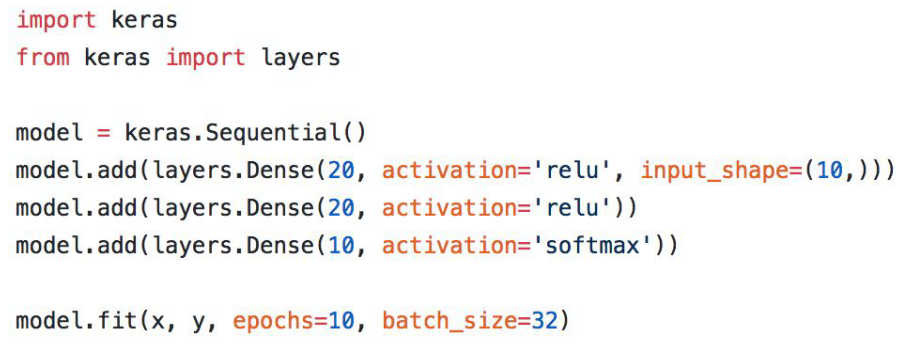
\includegraphics[width=\linewidth,keepaspectratio]{kr20}
\end{center}
\end{frame}

%%%%%%%%%%%%%%%%%%%%%%%%%%%%%%%%%%%%%%%%%%%%%%%%%%%
\begin{frame}[fragile] \frametitle{The functional API}
\begin{center}
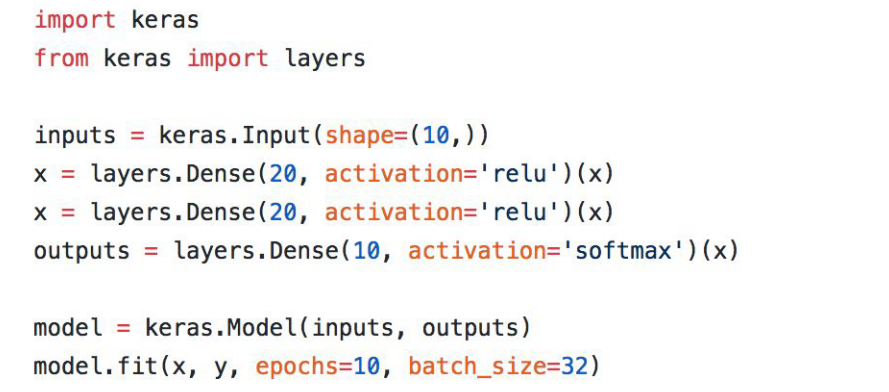
\includegraphics[width=\linewidth,keepaspectratio]{kr21}
\end{center}
\end{frame}

%%%%%%%%%%%%%%%%%%%%%%%%%%%%%%%%%%%%%%%%%%%%%%%%%%%
\begin{frame}[fragile] \frametitle{Model subclassing}
\begin{center}
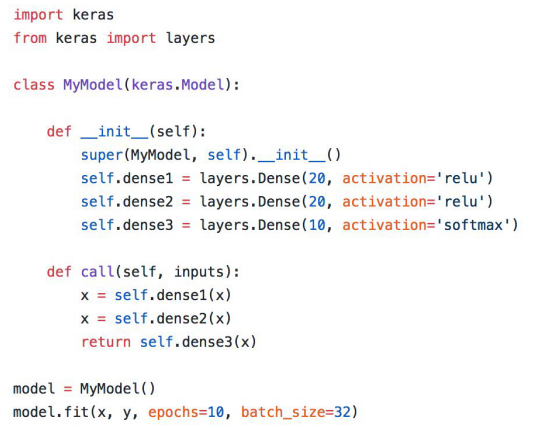
\includegraphics[width=\linewidth,keepaspectratio]{kr22}
\end{center}
\end{frame}

%%%%%%%%%%%%%%%%%%%%%%%%%%%%%%%%%%%%%%%%%%%%%%%%%%%
\begin{frame}[fragile] \frametitle{Understanding deferred (symbolic)
vs. eager (imperative)}

\begin{itemize}
\item  Deferred: you use Python to build a computation graph that gets executed later
\item  Eager: the Python runtime is the execution runtime (like Numpy)
\item Symbolic tensors don’t have a value in your Python code (yet)
\item  Eager tensors have a value in your Python code
\item With eager execution, you can use value-dependent dynamic topologies 
(tree-RNNs)
\end{itemize}
\end{frame}

%%%%%%%%%%%%%%%%%%%%%%%%%%%%%%%%%%%%%%%%%%%%%%%%%%%
\begin{frame}[fragile] \frametitle{Eager Execution}

The Keras functional API and Sequential API work with eager execution


\begin{center}
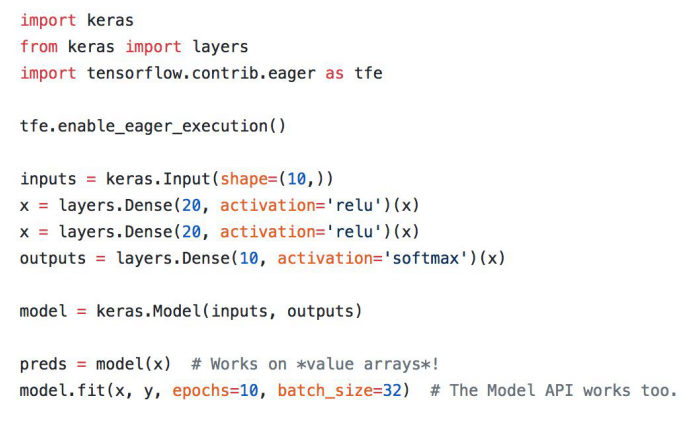
\includegraphics[width=\linewidth,keepaspectratio]{kr23}
\end{center}
\end{frame}


%%%%%%%%%%%%%%%%%%%%%%%%%%%%%%%%%%%%%%%%%%%%%%%%%%%
\begin{frame}[fragile] \frametitle{Eager Execution}

Eager execution allows you to write imperative custom layers


\begin{center}
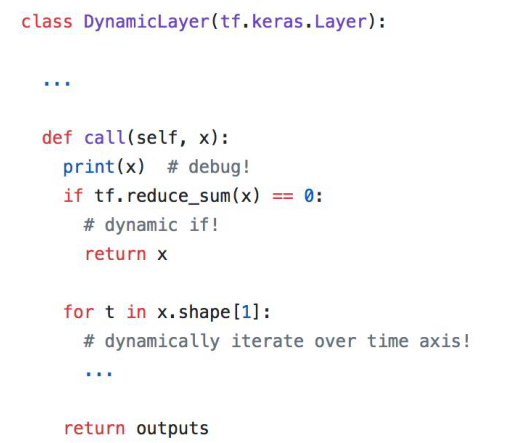
\includegraphics[width=0.65\linewidth,keepaspectratio]{kr24}
\end{center}
\end{frame}

%%%%%%%%%%%%%%%%%%%%%%%%%%%%%%%%%%%%%%%%%%%%%%%%%%%
\begin{frame}[fragile] \frametitle{Eager Execution}

Maximum flexibility: imperative Model subclassing

\begin{center}
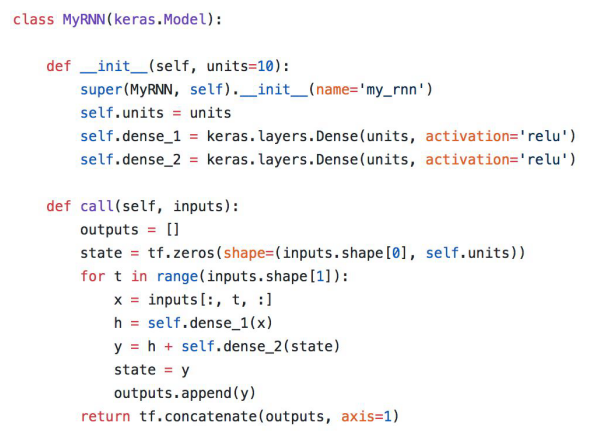
\includegraphics[width=0.8\linewidth,keepaspectratio]{kr25}
\end{center}
\end{frame}



%%%%%%%%%%%%%%%%%%%%%%%%%%%%%%%%%%%%%%%%%%%%%%%%%%%
\begin{frame}
  \begin{center}
    {\Large Sequential Workflow: more details}
    
  \end{center}
\end{frame}
%%%%%%%%%%%%%%%%%%%%%%%%%%%%%%%%%%%%%%%%%%%%%%%%%%%
\begin{frame}[fragile] \frametitle{Steps}

\begin{itemize}
\item  Prepare your 
input and 
output tensors 
\item  Create first 
layer to handle 
input layer
\item  Create last 
layer to handle 
output targets
\item Build any 
model you like 
in between
\end{itemize}
\end{frame}

%%%%%%%%%%%%%%%%%%%%%%%%%%%%%%%%%%%%%%%%%%%%%%%%%%%
\begin{frame}[fragile] \frametitle{Steps}
\begin{center}
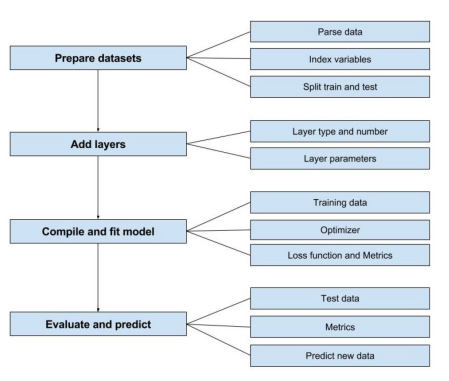
\includegraphics[width=0.65\linewidth,keepaspectratio]{kr2}
\end{center}
\end{frame}

%%%%%%%%%%%%%%%%%%%%%%%%%%%%%%%%%%%%%%%%%%%%%%%%%%%
\begin{frame}[fragile] \frametitle{Build Layers}
\begin{lstlisting}
from keras.models import Sequential
from keras.layers import Dense, Activation

model = Sequential()

model.add(Dense(units=64, input_dim=100))
model.add(Activation('relu'))
model.add(Dense(units=10))
model.add(Activation('softmax'))
\end{lstlisting}

\begin{itemize}
\item Constructing a Sequential model, and
adding three layers to it: a linear, or dense, layer;
the activation layer; and the output layer.
\begin{lstlisting}
>>> model = Sequential()
>>> model.add(Dense(512, input_shape=(28 * 28,)))
>>> model.add(Activation("sigmoid"))
>>> model.add(Dense(10))
\end{lstlisting}
\item The input shape parameter needs to be set for the
first layer, but can be inferred for all of the other
layers.
\end{itemize}
\end{frame}


%%%%%%%%%%%%%%%%%%%%%%%%%%%%%%%%%%%%%%%%%%%%%%%%%%%
\begin{frame}[fragile] \frametitle{Compile Model}
\begin{lstlisting}
model.compile(loss='categorical_crossentropy',optimizer='sgd',
metrics=['accuracy'])

or

model.compile(loss=keras.losses.categorical_crossentropy,optimizer=
keras.optimizers.SGD(lr=0.01, momentum=0.9))
\end{lstlisting}

\begin{itemize}
\item Compile the model (this may take a minute
or more) using stochastic gradient descent.
\begin{lstlisting}
>>> sgd = SGD(lr = 0.02, momentum = 0.01, nesterov = True)
>>> model.compile(loss='mse', optimizer=sgd)
\end{lstlisting}
\item By setting various environment variables, we could do this
over Tensorflow or Theano, and could make it run over
various CPU or GPU architectures.
\end{itemize}

\end{frame}

%%%%%%%%%%%%%%%%%%%%%%%%%%%%%%%%%%%%%%%%%%%%%%%%%%%
\begin{frame}[fragile] \frametitle{Training}
\begin{lstlisting}
model.fit(x_train, y_train, epochs=5, batch_size=32)

# You can feed data batches manually

model.train_on_batch(x_batch, y_batch)
\end{lstlisting}

\begin{itemize}
\item To train the actual model, we run the fit method on
the model, giving the desired batch size and number
of epochs:
\begin{lstlisting}
>>> model.fit(X_train, Y_train, batch_size=32, nb_epoch=25,
...           verbose=1, show_accuracy=True)
\end{lstlisting}
\item This will produce a running output of the model training
process.

% \item Run this is the Python interpreter
% and see the various advanced features than can be easily added
% to adapt the final model.
\end{itemize}
\end{frame}


%%%%%%%%%%%%%%%%%%%%%%%%%%%%%%%%%%%%%%%%%%%%%%%%%%%
\begin{frame}[fragile] \frametitle{Usage}
\begin{lstlisting}
# Evaluation

loss_and_metrics = model.evaluate(x_test, y_test, batch_size=128)

# Prediction

classes = model.predict(x_test, batch_size=128)
\end{lstlisting}

\end{frame}


% %%%%%%%%%%%%%%%%%%%%%%%%%%%%%%%%%%%%%%%%%%%%%%%%%%%
% \begin{frame}[fragile] \frametitle{Minimal working example}

% \begin{lstlisting}
% >>> from keras.models import Sequential
% >>> from keras.layers.core import Dense, Activation
% >>> from keras.optimizers import SGD
% \end{lstlisting}

% \end{frame}

% %%%%%%%%%%%%%%%%%%%%%%%%%%%%%%%%%%%%%%%%%%%%%%%%%%%
% \begin{frame}[fragile] \frametitle{Model Specification}

% \begin{itemize}
% \item Constructing a Sequential model, and
% adding three layers to it: a linear, or dense, layer;
% the activation layer; and the output layer.
% \begin{lstlisting}
% >>> model = Sequential()
% >>> model.add(Dense(512, input_shape=(28 * 28,)))
% >>> model.add(Activation("sigmoid"))
% >>> model.add(Dense(10))
% \end{lstlisting}
% \item The input shape parameter needs to be set for the
% first layer, but can be inferred for all of the other
% layers.
% \end{itemize}
% % \end{frame}

% %%%%%%%%%%%%%%%%%%%%%%%%%%%%%%%%%%%%%%%%%%%%%%%%%%%
% \begin{frame}[fragile] \frametitle{Model Compilation}

% \begin{itemize}
% \item Compile the model (this may take a minute
% or more) using stochastic gradient descent.
% \begin{lstlisting}
% >>> sgd = SGD(lr = 0.02, momentum = 0.01, nesterov = True)
% >>> model.compile(loss='mse', optimizer=sgd)
% \end{lstlisting}
% \item By setting various environment variables, we could do this
% over Tensorflow or Theano, and could make it run over
% various CPU or GPU architectures.
% \end{itemize}
% \end{frame}

% %%%%%%%%%%%%%%%%%%%%%%%%%%%%%%%%%%%%%%%%%%%%%%%%%%%
% \begin{frame}[fragile] \frametitle{Model Fitting}

% \begin{itemize}
% \item To train the actual model, we run the fit method on
% the model, giving the desired batch size and number
% of epochs:
% \begin{lstlisting}
% >>> model.fit(X_train, Y_train, batch_size=32, nb_epoch=25,
% ...           verbose=1, show_accuracy=True)
% \end{lstlisting}
% \item This will produce a running output of the model training
% process.

% \item Run this is the Python interpreter
% and see the various advanced features than can be easily added
% to adapt the final model.
% \end{itemize}
% \end{frame}

%%%%%%%%%%%%%%%%%%%%%%%%%%%%%%%%%%%%%%%%%%%%%%%%%%%
\begin{frame}[fragile] \frametitle{Terminologies}

In the neural network terminology:

\begin{itemize}
\item one epoch = one forward pass and one backward pass of all the training examples
\item batch size = the number of training examples in one forward/backward pass. The higher the batch size, the more memory space you'll need.
\item number of iterations = number of passes, each pass using [batch size] number of examples. To be clear, one pass = one forward pass + one backward pass (we do not count the forward pass and backward pass as two different passes).
\item Example: if you have 1000 training examples, and your batch size is 500, then it will take 2 iterations to complete 1 epoch.
\end{itemize}
\end{frame}

%%%%%%%%%%%%%%%%%%%%%%%%%%%%%%%%%%%%%%%%%%%%%%%%%%%
\begin{frame}[fragile] \frametitle{Terminologies: Layers Parameters}

Keras Layers Shape parameters

\begin{itemize}
\item Units: number of neurons. Output shape. Its a property of each layer.
\item Input Shape: In Keras, there is no input layer. Its a tensor. It goes to the first hidden layer. This tensor must have the same shape as your training data. Example: if you have 30 images of 50x50 pixels in RGB (3 channels), the shape of your input data is (30,50,50,3). Then your input layer tensor, must have this shape. (See next slide for more info on input shapes)
\item Now, the input shape is the only one you must define, because your model cannot know it. Only you know that, based on your training data.

\item All the other shapes are calculated automatically based on the units and particularities of each layer.
\item Since the input shape is the only one you need to define, Keras will demand it in the first layer.
\end{itemize}

\tiny{(Ref: Keras input explanation: input\_shape, units, batch\_size, dim, etc - Stack Overflow)}
\end{frame}

%%%%%%%%%%%%%%%%%%%%%%%%%%%%%%%%%%%%%%%%%%%%%%%%%%%
\begin{frame}[fragile] \frametitle{Terminologies: Input Shapes}

Each type of layer requires the input with a certain number of dimensions:

\begin{itemize}
\item Dense layers have output shape based on "units". Dense layers require inputs as (batch\_size, input\_size) or (batch\_size, optional,...,optional, input\_size)
\item Convolutional layers have output shape based on "filters". But it's always based on some layer property. 
\item 2D convolutional layers need inputs as:
\begin{itemize}
\item if using channels\_last: (batch\_size, imageside1, imageside2, channels)
\item if using channels\_first: (batch\_size, channels, imageside1, imageside2)
\end{itemize}
\item 1D convolutions and recurrent layers use (batch\_size, sequence\_length, features)
\end{itemize}

\tiny{(Ref: Keras input explanation: input\_shape, units, batch\_size, dim, etc - Stack Overflow)}
\end{frame}

%%%%%%%%%%%%%%%%%%%%%%%%%%%%%%%%%%%%%%%%%%%%%%%%%%%
\begin{frame}[fragile] \frametitle{Terminologies: Input Shapes}

As such, the following three snippets are strictly equivalent:

\begin{lstlisting}
model = Sequential()
model.add(Dense(32, input_shape=(784,)))
\end{lstlisting}

\begin{lstlisting}
model = Sequential()
model.add(Dense(32, batch_input_shape=(None, 784)))
# note that batch dimension is "None" here,
# so the model will be able to process batches of any size.
\end{lstlisting}

\begin{lstlisting}
model = Sequential()
model.add(Dense(32, input_dim=784))
\end{lstlisting}

\tiny{(Ref: Specifying the input shape - Keras Documentation)}
\end{frame}



%%%%%%%%%%%%%%%%%%%%%%%%%%%%%%%%%%%%%%%%%%%%%%%%%%%
\begin{frame}[fragile] \frametitle{Terminologies: Input Shapes}

And so are the following three snippets:

\begin{lstlisting}
model = Sequential()
model.add(LSTM(32, input_shape=(10, 64)))
\end{lstlisting}

\begin{lstlisting}
model = Sequential()
model.add(LSTM(32, batch_input_shape=(None, 10, 64)))
\end{lstlisting}

\begin{lstlisting}
model = Sequential()
model.add(LSTM(32, input_length=10, input_dim=64))
\end{lstlisting}

\tiny{(Ref: Specifying the input shape - Keras Documentation)}
\end{frame}


%%%%%%%%%%%%%%%%%%%%%%%%%%%%%%%%%%%%%%%%%%%%%%%%%%%
\begin{frame}[fragile] \frametitle{Terminologies: Shapes}

\begin{itemize}
\item Example: 30 images, 50x50 pixels and 3 channels, having an input shape of (30,50,50,3).
\item But in this definition, Keras ignores the first dimension, which is the batch size. Your model should be able to deal with any batch size, so you define only the other dimensions: \lstinline|input_shape = (50,50,3) #regardless of how many images I have, each image has this shape|
\item But if you want to pass batch size (or required by certain models)  then \lstinline|batch_input_shape=(30,50,50,3) or batch_shape=(30,50,50,3)|
\item Either way you choose, tensors in the model will have the batch dimension.
\item So, even if you used input\_shape=(50,50,3), when keras sends you messages, or when you print the model summary, it will show (None,50,50,3).
\item The first dimension is the batch size, it's None because it can vary depending on how many examples you give for training. (If you defined the batch size explicitly, then the number you defined will appear instead of None)
\end{itemize}

\tiny{(Ref: Keras input explanation: input\_shape, units, batch\_size, dim, etc - Stack Overflow)}
\end{frame}


%%%%%%%%%%%%%%%%%%%%%%%%%%%%%%%%%%%%%%%%%%%%%%%%%%%
\begin{frame}[fragile] \frametitle{Terminologies: The output shape}

Relation between shapes and units

\begin{itemize}
\item Given the input shape, all other shapes are results of layers calculations.
\item The "units" of each layer will define the output shape
\item A dense layer has an output shape of (batch\_size,units)
\item Weights will be entirely automatically calculated based on the input and the output shapes.
\item In a dense layer, weights multiply all inputs. It's a matrix with one column per input and one row per unit
\end{itemize}

\tiny{(Ref: Keras input explanation: input\_shape, units, batch\_size, dim, etc - Stack Overflow)}
\end{frame}


%%%%%%%%%%%%%%%%%%%%%%%%%%%%%%%%%%%%%%%%%%%%%%%%%%%
\begin{frame}[fragile] \frametitle{Terminologies: Dim}

What is dim?

\begin{itemize}
\item If your input shape has only one dimension, you don't need to give it as a tuple, you give input\_dim as a scalar number.
\item So, in your model, where your input layer has 3 elements, you can use any of these two:
\begin{itemize}
\item input\_shape=(3,) -- The comma is necessary when you have only one dimension
\item input\_dim = 3
\end{itemize}
\item But when dealing directly with the tensors, often dim will refer to how many dimensions a tensor has. For instance a tensor with shape (25,10909) has 2 dimensions.
\end{itemize}

\tiny{(Ref: Keras input explanation: input\_shape, units, batch\_size, dim, etc - Stack Overflow)}
\end{frame}

%%%%%%%%%%%%%%%%%%%%%%%%%%%%%%%%%%%%%%%%%%%%%%%%%%%
\begin{frame}[fragile] \frametitle{Example: Images}

With the Sequential model:

\begin{lstlisting}
from keras.models import Sequential  
from keras.layers import *  

model = Sequential()    

#start from the first hidden layer, since the input is not actually a layer   
#but inform the shape of the input, with 3 elements.    
model.add(Dense(units=4,input_shape=(3,))) #hidden layer 1 with input

#further layers:    
model.add(Dense(units=4)) #hidden layer 2
model.add(Dense(units=1)) #output layer   
\end{lstlisting}

\tiny{(Ref: Keras input explanation: input\_shape, units, batch\_size, dim, etc - Stack Overflow)}
\end{frame}

%%%%%%%%%%%%%%%%%%%%%%%%%%%%%%%%%%%%%%%%%%%%%%%%%%%
\begin{frame}[fragile] \frametitle{Example: Images}

With the functional API Model:

\begin{lstlisting}
from keras.models import Model   
from keras.layers import * 

#Start defining the input tensor:
inpTensor = Input((3,))   

#create the layers and pass them the input tensor to get the output tensor:    
hidden1Out = Dense(units=4)(inpTensor)    
hidden2Out = Dense(units=4)(hidden1Out)    
finalOut = Dense(units=1)(hidden2Out)   

#define the model's start and end points    
model = Model(inpTensor,finalOut)  
\end{lstlisting}

Remember you ignore batch sizes when defining layers:

\begin{itemize}
\item  inpTensor: (None,3)
\item  hidden1Out: (None,4)
\item  hidden2Out: (None,4)
\item  finalOut: (None,1)
\end{itemize}


\tiny{(Ref: Keras input explanation: input\_shape, units, batch\_size, dim, etc - Stack Overflow)}
\end{frame}


%%%%%%%%%%%%%%%%%%%%%%%%%%%%%%%%%%%%%%%%%%%%%%%%%%%
\begin{frame}
  \begin{center}
    {\Large Keras Binary Classification: Step by Step}
    
    \tiny{(Ref:  Develop Your First Neural Network in Python With Keras Step-By-Step, Jason Brownlee)}
  \end{center}
\end{frame}

%%%%%%%%%%%%%%%%%%%%%%%%%%%%%%%%%%%%%%%%%%%%%%%%%%%
\begin{frame}[fragile] \frametitle{Tutorial Overview}
Steps:
\begin{itemize}
\item  Load Data.
\item  Define Model.
\item  Compile Model.
\item  Fit Model.
\item  Evaluate Model.
\item  Tie It All Together.

\end{itemize}
\end{frame}

%%%%%%%%%%%%%%%%%%%%%%%%%%%%%%%%%%%%%%%%%%%%%%%%%%%
\begin{frame}[fragile] \frametitle{Imports}
Note: machine learning algorithms that use a stochastic process (e.g. random numbers), it is a good idea to set the random number seed.
\begin{lstlisting}
from keras.models import Sequential
from keras.layers import Dense
import numpy
# fix random seed for reproducibility
numpy.random.seed(7)
\end{lstlisting}
\end{frame}

%%%%%%%%%%%%%%%%%%%%%%%%%%%%%%%%%%%%%%%%%%%%%%%%%%%
\begin{frame}[fragile] \frametitle{Data set}
 \begin{itemize}
 \item  Download the Pima Indian dataset from the UCI Machine Learning repository http://archive.ics.uci.edu/ml/machine-learning-databases/pima-indians-diabetes/pima-indians-diabetes.data 
\item  It describes patient medical record data for Pima Indians and whether they had an onset of diabetes within five years.
\item  It is a binary classification problem (onset of diabetes as 1 or not as 0). 
\item All of the input variables that describe each patient are numerical. 
\item This makes it easy to use directly with neural networks that expect numerical input and output values
\end{itemize}
\end{frame}

%%%%%%%%%%%%%%%%%%%%%%%%%%%%%%%%%%%%%%%%%%%%%%%%%%%
\begin{frame}[fragile] \frametitle{Load Data}
 \begin{itemize}
\item  There are eight input variables and one output variable (the last column).
\item Once loaded we can split the dataset into input variables (X) and the output class variable (Y).
\end{itemize}
\begin{lstlisting}
# load pima indians dataset
dataset = numpy.loadtxt("pima-indians-diabetes.csv", delimiter=",")
# split into input (X) and output (Y) variables
X = dataset[:,0:8]
Y = dataset[:,8]
\end{lstlisting}
\end{frame}

%%%%%%%%%%%%%%%%%%%%%%%%%%%%%%%%%%%%%%%%%%%%%%%%%%%
\begin{frame}[fragile] \frametitle{Define Model: Input}
 \begin{itemize}
\item  Models in Keras are defined as a sequence of layers.
\item We create a Sequential model and add layers one at a time.
\item The first thing to get right is to ensure the input layer has the right number of inputs. 
\item This can be specified when creating the first layer with the input\_dim argument and setting it to 8 for the 8 input variables.
\end{itemize}
\end{frame}

%%%%%%%%%%%%%%%%%%%%%%%%%%%%%%%%%%%%%%%%%%%%%%%%%%%
\begin{frame}[fragile] \frametitle{Define Model: Layers}
 \begin{itemize}
\item  How do we know the number of layers and their types?
\item Use Heuristics, trial and error, experience.
\item Here, we will use a fully-connected network structure with three layers.

\end{itemize}
\end{frame}


%%%%%%%%%%%%%%%%%%%%%%%%%%%%%%%%%%%%%%%%%%%%%%%%%%%
\begin{frame}[fragile] \frametitle{Define Model: Dense Layers}
 \begin{itemize}
\item  Fully connected layers are defined using the Dense class. 
\item We can specify the number of neurons in the layer as the first argument, the initialization method as the second argument as init and specify the activation function using the activation argument.
\end{itemize}
\end{frame}


%%%%%%%%%%%%%%%%%%%%%%%%%%%%%%%%%%%%%%%%%%%%%%%%%%%
\begin{frame}[fragile] \frametitle{Define Model: Dense Layers Weights}
 \begin{itemize}
\item  We initialize the network weights to a small random number generated from a uniform distribution (`uniform'), in this case between 0 and 0.05 because that is the default uniform weight initialization in Keras. 
\item Another traditional alternative would be `normal' for small random numbers generated from a Gaussian distribution.
\end{itemize}
\end{frame}

%%%%%%%%%%%%%%%%%%%%%%%%%%%%%%%%%%%%%%%%%%%%%%%%%%%
\begin{frame}[fragile] \frametitle{Define Model: Dense Layers Activations}
 \begin{itemize}
\item  We will use the rectifier (`relu') activation function on the first two layers and the sigmoid function in the output layer.
\item It used to be the case that sigmoid and tanh activation functions were preferred for all layers. 
\item These days, better performance is achieved using the rectifier activation function. 
\item We use a sigmoid on the output layer to ensure our network output is between 0 and 1 and easy to map to either a probability of class 1 or snap to a hard classification of either class with a default threshold of 0.5.
\end{itemize}
\end{frame}


%%%%%%%%%%%%%%%%%%%%%%%%%%%%%%%%%%%%%%%%%%%%%%%%%%%
\begin{frame}[fragile] \frametitle{Define Model: Dense Layers}
 \begin{itemize}
\item  The first layer has 12 neurons and expects 8 input variables. 
\item The second hidden layer has 8 neurons and finally,
\item the output layer has 1 neuron to predict the class (onset of diabetes or not).
\end{itemize}
\begin{lstlisting}
# create model
model = Sequential()
model.add(Dense(12, input_dim=8, activation='relu'))
model.add(Dense(8, activation='relu'))
model.add(Dense(1, activation='sigmoid'))
\end{lstlisting}
\end{frame}


%%%%%%%%%%%%%%%%%%%%%%%%%%%%%%%%%%%%%%%%%%%%%%%%%%%
\begin{frame}[fragile] \frametitle{Compile Model}
 \begin{itemize}
\item  When compiling, we must specify some additional properties required when training the network. 
\item Remember training a network means finding the best set of weights to make predictions for this problem.
\item We must specify the loss function to use to evaluate a set of weights, the optimizer used to search through different weights for the network and any optional metrics we would like to collect and report during training.
\end{itemize}
\end{frame}

%%%%%%%%%%%%%%%%%%%%%%%%%%%%%%%%%%%%%%%%%%%%%%%%%%%
\begin{frame}[fragile] \frametitle{Compile Model}
 \begin{itemize}
\item We will use logarithmic loss, which for a binary classification problem is defined in Keras as ``binary\_crossentropy''. 
\item We will also use the efficient gradient descent algorithm ``adam'' for no other reason that it is an efficient default. 
\item Note: No data has yet been provided to FIT the model
\item We compiled it just to be ready for efficient computation.
\end{itemize}
\begin{lstlisting}
# Compile model
model.compile(loss='binary_crossentropy', optimizer='adam', metrics=['accuracy'])
\end{lstlisting}
\end{frame}

%%%%%%%%%%%%%%%%%%%%%%%%%%%%%%%%%%%%%%%%%%%%%%%%%%%
\begin{frame}[fragile] \frametitle{Fit Model}
 \begin{itemize}
\item Will run for a fixed number of iterations through the dataset called epochs, nepochs
\item Can also set the number of instances that are evaluated before a weight update in the network is performed, called the batch size and set using the batch\_size argument.
\item Both are to be chosen by heiristics, trial and error or by experince
\item Will run for a small number of iterations (150) and use a relatively small batch size of 10
\end{itemize}
\begin{lstlisting}
# Fit the model
model.fit(X, Y, epochs=150, batch_size=10)
\end{lstlisting}
\end{frame}


%%%%%%%%%%%%%%%%%%%%%%%%%%%%%%%%%%%%%%%%%%%%%%%%%%%
\begin{frame}[fragile] \frametitle{Evaluate Model}
 \begin{itemize}
\item We have trained our neural network on the entire dataset and we can evaluate the performance of the network on the same dataset (for simplicity)
\item Ideally another labelled data should have been used for testing (or some Cross Validation within Training dataset)
\end{itemize}
\begin{lstlisting}
# evaluate the model
scores = model.evaluate(X, Y)
print("\n{}: {}".format(model.metrics_names[1], scores[1]*100))
\end{lstlisting}
\end{frame}

%%%%%%%%%%%%%%%%%%%%%%%%%%%%%%%%%%%%%%%%%%%%%%%%%%%
\begin{frame}[fragile] \frametitle{Make Predictions}
 \begin{itemize}
\item Use the fitted model to generate predictions on the training dataset, pretending it is a new dataset we have not seen before.
\item For now, using X itself
\end{itemize}
\begin{lstlisting}
# calculate predictions
predictions = model.predict(X)
# round predictions
rounded = [round(x[0]) for x in predictions]
print(rounded)

[1.0, 0.0, ... 1.0, 0.0]
\end{lstlisting}
\end{frame}


%%%%%%%%%%%%%%%%%%%%%%%%%%%%%%%%%%%%%%%%%%%%%%%%%%%
\begin{frame}
  \begin{center}
    {\Large Keras Mutliclass Classification: Step by Step}
    
    \tiny{(Ref:  Multi-Class Classification Tutorial with the Keras Deep Learning Library - Jason Brownlee)}
  \end{center}
\end{frame}


%%%%%%%%%%%%%%%%%%%%%%%%%%%%%%%%%%%%%%%%%%%%%%%%%%%
\begin{frame}[fragile] \frametitle{Data set}
 \begin{itemize}
 \item  Iris flower dataset http://archive.ics.uci.edu/ml/datasets/Iris
 \item  4 input variables are numeric and have the same scale in centimeters. 
 \item Each instance describes the properties of an observed flower measurements and the output variable is specific iris species.
 \item This is a multi-class classification problem, meaning that there are more than two classes to be predicted, in fact there are three flower species.
\end{itemize}
\end{frame}

%%%%%%%%%%%%%%%%%%%%%%%%%%%%%%%%%%%%%%%%%%%%%%%%%%%
\begin{frame}[fragile] \frametitle{Imports}
\begin{lstlisting}
import numpy
import pandas
from keras.models import Sequential
from keras.layers import Dense
from keras.wrappers.scikit_learn import KerasClassifier
from keras.utils import np_utils
from sklearn.model_selection import cross_val_score
from sklearn.model_selection import KFold
from sklearn.preprocessing import LabelEncoder
from sklearn.pipeline import Pipeline

# fix random seed for reproducibility
seed = 7
numpy.random.seed(seed)
\end{lstlisting}
\end{frame}

%%%%%%%%%%%%%%%%%%%%%%%%%%%%%%%%%%%%%%%%%%%%%%%%%%%
\begin{frame}[fragile] \frametitle{Load Data}
 \begin{itemize}
 \item  The dataset can be loaded directly. 
 \item Because the output variable contains strings, it is easiest to load the data using pandas. 
 \item We can then split the attributes (columns) into input variables (X) and output variables (Y).
 \end{itemize}
\begin{lstlisting}
# load dataset
dataframe = pandas.read_csv("iris.csv", header=None)
dataset = dataframe.values
X = dataset[:,0:4].astype(float)
Y = dataset[:,4]
\end{lstlisting}
\end{frame}

%%%%%%%%%%%%%%%%%%%%%%%%%%%%%%%%%%%%%%%%%%%%%%%%%%%
\begin{frame}[fragile] \frametitle{ Encode Output}
 \begin{itemize}
 \item  The output variable contains three different string values.
 \item Need One Hot Encoding or creating dummy variables from a categorical variable
 \item For example, in this problem three class values are Iris-setosa, Iris-versicolor and Iris-virginica
 \item We can turn this into a one-hot encoded binary matrix for each data instance that would look as follows:
 \end{itemize}
\end{frame}

%%%%%%%%%%%%%%%%%%%%%%%%%%%%%%%%%%%%%%%%%%%%%%%%%%%
\begin{frame}[fragile] \frametitle{ Encode Output}
\begin{lstlisting}
# encode class values as integers
encoder = LabelEncoder()
encoder.fit(Y)
encoded_Y = encoder.transform(Y)
# convert integers to dummy variables (i.e. one hot encoded)
dummy_y = np_utils.to_categorical(encoded_Y)

Iris-setosa,	Iris-versicolor,	Iris-virginica
1,		0,			0
0,		1, 			0
0, 		0, 			1
\end{lstlisting}
\end{frame}

%%%%%%%%%%%%%%%%%%%%%%%%%%%%%%%%%%%%%%%%%%%%%%%%%%%
\begin{frame}[fragile] \frametitle{ Define Model}
 \begin{itemize}
 \item  Create a simple fully connected network with one hidden layer that contains 8 neurons.
 \item The hidden layer uses a rectifier activation function
 \item Due to 3 valued One hot encoding, the output layer must create 3 output values, one for each class. 
 \item The output value with the largest value will be taken as the class predicted by the model.
 \item The network topology of this simple one-layer neural network can be summarized as:
 \end{itemize}
 \begin{lstlisting}
4 inputs -> [8 hidden nodes] -> 3 outputs
\end{lstlisting}
\end{frame}

%%%%%%%%%%%%%%%%%%%%%%%%%%%%%%%%%%%%%%%%%%%%%%%%%%%
\begin{frame}[fragile] \frametitle{ Define Model}
 \begin{itemize}
 \item  Softmax at the end layer,  to ensure the output values are in the range of 0 and 1 and may be used as predicted probabilities.
 \item Use the efficient Adam gradient descent optimization algorithm with a logarithmic loss function, which is called ``categorical\_crossentropy'' in Keras.
 \end{itemize}
 \begin{lstlisting}
# define baseline model
def baseline_model():
	# create model
	model = Sequential()
	model.add(Dense(8, input_dim=4, activation='relu'))
	model.add(Dense(3, activation='softmax'))
	# Compile model
	model.compile(loss='categorical_crossentropy', optimizer='adam', metrics=['accuracy'])
	return model
\end{lstlisting}
\end{frame}


%%%%%%%%%%%%%%%%%%%%%%%%%%%%%%%%%%%%%%%%%%%%%%%%%%%
\begin{frame}[fragile] \frametitle{KerasClassifier}
 \begin{itemize}
 \item  This neural network model can be used in Scikit Learn to leverage ML facilities there.
 \item Create our KerasClassifier for use in scikit-learn
 \item KerasClassifier takes the name of a function as an argument. 
 \item This function (called ``baseline\_model'' here) must return the constructed neural network model, ready for training.
 \end{itemize}
 \begin{lstlisting}
estimator = KerasClassifier(build_fn=baseline_model, epochs=200, batch_size=5, verbose=0)
\end{lstlisting}
\end{frame}

%%%%%%%%%%%%%%%%%%%%%%%%%%%%%%%%%%%%%%%%%%%%%%%%%%%
\begin{frame}[fragile] \frametitle{Evaluate with k-Fold Cross Validation}
 \begin{itemize}
 \item  The scikit-learn has excellent capability to evaluate models using a suite of techniques, like K-Fold cross validation
 \item We can evaluate our model (estimator) on our dataset (X and dummy\_y) using a 10-fold cross-validation procedure (kfold).
 \end{itemize}
 \begin{lstlisting}
 kfold = KFold(n_splits=10, shuffle=True, random_state=seed)
results = cross_val_score(estimator, X, dummy_y, cv=kfold)
print("Accuracy: {}\% ({}\%)".format(results.mean()*100, results.std()*100))
\end{lstlisting}
\end{frame}

%%%%%%%%%%%%%%%%%%%%%%%%%%%%%%%%%%%%%%%%%%%%%%%%%%%
\begin{frame}[fragile] \frametitle{Results}
 \begin{itemize}
 \item  The results are summarized as both the mean and standard deviation of the model accuracy on the dataset.
 \item  This is a reasonable estimation of the performance of the model on unseen data.
 \end{itemize}
 \begin{lstlisting}
Accuracy: 97.33% (4.42%)
\end{lstlisting}
\end{frame}

%%%%%%%%%%%%%%%%%%%%%%%%%%%%%%%%%%%%%%%%%%%%%%%%%%%
\begin{frame}
  \begin{center}
    {\Large Keras Regression: Step by Step}
    
    \tiny{(Ref:  Regression Tutorial with the Keras Deep Learning Library in Python, Jason Brownlee)}
  \end{center}
\end{frame}


%%%%%%%%%%%%%%%%%%%%%%%%%%%%%%%%%%%%%%%%%%%%%%%%%%%
\begin{frame}[fragile] \frametitle{Data set}
 \begin{itemize}
 \item   Boston house price dataset : https://archive.ics.uci.edu/ml/datasets/Housing
 \item  The dataset describes 13 numerical properties of houses in Boston suburbs and is concerned with modeling the price of houses in those suburbs in thousands of dollars. 
 \item As such, this is a regression predictive modeling problem. 
 \item Input attributes include things like crime rate, proportion of nonretail business acres, chemical concentrations and more.
\end{itemize}
\end{frame}

%%%%%%%%%%%%%%%%%%%%%%%%%%%%%%%%%%%%%%%%%%%%%%%%%%%
\begin{frame}[fragile] \frametitle{Imports}
\begin{lstlisting}
import numpy
import pandas
from keras.models import Sequential
from keras.layers import Dense
from keras.wrappers.scikit_learn import KerasRegressor
from sklearn.model_selection import cross_val_score
from sklearn.model_selection import KFold
from sklearn.preprocessing import StandardScaler
from sklearn.pipeline import Pipeline
\end{lstlisting}
\end{frame}

%%%%%%%%%%%%%%%%%%%%%%%%%%%%%%%%%%%%%%%%%%%%%%%%%%%
\begin{frame}[fragile] \frametitle{Load Data}
 \begin{itemize}
 \item The dataset is in fact not in CSV format, instead separated by whitespace. 
 \item We can then split the input (X) and output (Y) attributes
 \end{itemize}
\begin{lstlisting}
# load dataset
dataframe = pandas.read_csv("housing.csv", delim_whitespace=True, header=None)
dataset = dataframe.values
# split into input (X) and output (Y) variables
X = dataset[:,0:13]
Y = dataset[:,13]
\end{lstlisting}
\end{frame}


%%%%%%%%%%%%%%%%%%%%%%%%%%%%%%%%%%%%%%%%%%%%%%%%%%%
\begin{frame}[fragile] \frametitle{Keras Regressor}
 \begin{itemize}
 \item Scikit-learn excels at evaluating models and will allow us to use powerful data preparation and model evaluation schemes with very few lines of code.
 \item The Keras wrappers require a function as an argument. This function that we must define is responsible for creating the neural network model to be evaluated.
 \item No activation function is used for the output layer because it is a regression problem and we are interested in predicting numerical values directly without transform.
 \end{itemize}
\end{frame}


%%%%%%%%%%%%%%%%%%%%%%%%%%%%%%%%%%%%%%%%%%%%%%%%%%%
\begin{frame}[fragile] \frametitle{Keras Regressor}
 \begin{lstlisting}
def baseline_model():
	# create model
	model = Sequential()
	model.add(Dense(13, input_dim=13, kernel_initializer='normal', activation='relu'))
	model.add(Dense(1, kernel_initializer='normal'))
	# Compile model
	model.compile(loss='mean_squared_error', optimizer='adam')
	return model
\end{lstlisting}
\end{frame}


%%%%%%%%%%%%%%%%%%%%%%%%%%%%%%%%%%%%%%%%%%%%%%%%%%%
\begin{frame}[fragile] \frametitle{Keras Regressor}
 \begin{itemize}
 \item The Keras wrapper object for use in scikit-learn as a regression estimator is called KerasRegressor. 
 \item We create an instance and pass it both the name of the function to create the neural network model as well as some parameters to pass along to the fit() function of the model later, such as the number of epochs and batch size.
 \end{itemize}
\begin{lstlisting}
# fix random seed for reproducibility
seed = 7
numpy.random.seed(seed)
# evaluate model with standardized dataset
estimator = KerasRegressor(build_fn=baseline_model, nb_epoch=100, batch_size=5, verbose=0)
\end{lstlisting}
\end{frame}


%%%%%%%%%%%%%%%%%%%%%%%%%%%%%%%%%%%%%%%%%%%%%%%%%%%
\begin{frame}[fragile] \frametitle{Keras Regressor}
 \begin{itemize}
 \item The Keras wrapper object for use in scikit-learn as a regression estimator is called KerasRegressor. 
 \item We create an instance and pass it both the name of the function to create the neural network model as well as some parameters to pass along to the fit() function of the model later, such as the number of epochs and batch size.
 \end{itemize}
\begin{lstlisting}
# fix random seed for reproducibility
seed = 7
numpy.random.seed(seed)
# evaluate model with standardized dataset
estimator = KerasRegressor(build_fn=baseline_model, nb_epoch=100, batch_size=5, verbose=0)
\end{lstlisting}
\end{frame}

%%%%%%%%%%%%%%%%%%%%%%%%%%%%%%%%%%%%%%%%%%%%%%%%%%%
\begin{frame}[fragile] \frametitle{Results}
The final step is to evaluate this baseline model. We will use 10-fold cross validation to evaluate the model.
\begin{lstlisting}
kfold = KFold(n_splits=10, random_state=seed)
results = cross_val_score(estimator, X, Y, cv=kfold)
print("Results: {}({}) MSE".format(results.mean(), results.std()))

Results: 31.64 (26.82) MSE
\end{lstlisting}
\end{frame}



% %%%%%%%%%%%%%%%%%%%%%%%%%%%%%%%%%%%%%%%%%%%%%%%%%%%
% \begin{frame}
  % \begin{center}
    % {\Large Keras: In Depth}
    
    % {Ref: Deep Learning using Keras- alyosamah}
  % \end{center}
% \end{frame}

% %%%%%%%%%%%%%%%%%%%%%%%%%%%%%%%%%%%%%%%%%%%%%%%%%%%
% \begin{frame}[fragile] \frametitle{Sequential Models}
% \begin{center}
% 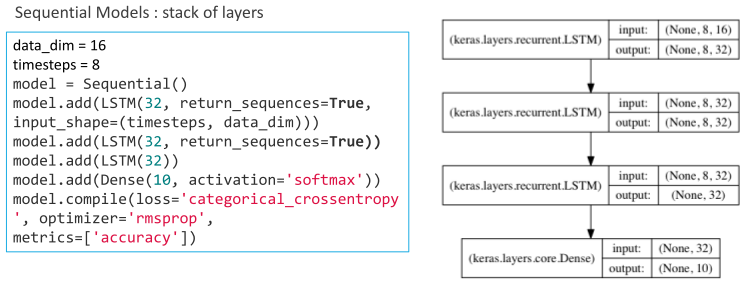
\includegraphics[width=\linewidth,keepaspectratio]{kr3}
% \end{center}
% \end{frame}

% %%%%%%%%%%%%%%%%%%%%%%%%%%%%%%%%%%%%%%%%%%%%%%%%%%%
% \begin{frame}[fragile] \frametitle{Keras Models}
 % Model Class API
% \begin{itemize}
% \item Optimized over all outputs Graph model 
% \item Allows for two or more independent networks to diverge or 
% merge 
% \item Allows for multiple separate inputs or outputs 
% \item Different merging layers (sum or concatenate)
% \end{itemize}
% \begin{lstlisting}
% from keras.models import Model 
% from keras.layers import Input, Dense 

% a = Input(shape=(32,)) 
% b = Dense(32)(a) 
% model = Model(inputs=a, outputs=b)
% \end{lstlisting}
% \end{frame}

% %%%%%%%%%%%%%%%%%%%%%%%%%%%%%%%%%%%%%%%%%%%%%%%%%%%
% \begin{frame}[fragile] \frametitle{Keras Layers}
% Layers are used to define what your architecture. Examples of layers are:
% \begin{itemize}
% \item  Dense layers (this is the normal, fully-connected 
% layer)
% \item  Convolutional layers (applies convolution operations on the previous layer)
% \item  Pooling layers (used after convolutional layers)
% \item  Dropout layers (these are used for regularization, to avoid overfitting)
% \end{itemize}
% \end{frame}

% %%%%%%%%%%%%%%%%%%%%%%%%%%%%%%%%%%%%%%%%%%%%%%%%%%%
% \begin{frame}[fragile] \frametitle{Keras Layers}
% Keras has a number of pre-built layers. Notable examples include: Regular dense, MLP type
% \begin{lstlisting}
% keras.layers.core.Dense(units, activation=None, use_bias=True, kernel_initializer='glorot_uniform', 
% bias_initializer='zeros', kernel_regularizer=None, bias_regularizer=None, activity_regularizer=None, 
% kernel_constraint=None, bias_constraint=None)
% \end{lstlisting}

% \end{frame}

% %%%%%%%%%%%%%%%%%%%%%%%%%%%%%%%%%%%%%%%%%%%%%%%%%%%
% \begin{frame}[fragile] \frametitle{Keras Layers}
% Recurrent layers, LSTM, GRU, etc

% \begin{lstlisting}
% keras.layers.recurrent.LSTM(units, activation='tanh', recurrent_activation='hard_sigmoid', 
% use_bias=True, kernel_initializer='glorot_uniform', recurrent_initializer='orthogonal', 
% bias_initializer='zeros', unit_forget_bias=True, kernel_regularizer=None, recurrent_regularizer=None, 
% bias_regularizer=None, activity_regularizer=None, kernel_constraint=None, recurrent_constraint=None, 
% bias_constraint=None, dropout=0.0, recurrent_dropout=0.0)
% \end{lstlisting}

% \end{frame}

% %%%%%%%%%%%%%%%%%%%%%%%%%%%%%%%%%%%%%%%%%%%%%%%%%%%
% \begin{frame}[fragile] \frametitle{Keras Layers}
% 2D Convolutional layers 

% \begin{lstlisting}
% keras.layers.convolutional.Conv2D(filters, kernel_size, strides=(1, 1), padding='valid', 
% data_format=None, dilation_rate=(1, 1), activation=None, use_bias=True, 
% kernel_initializer='glorot_uniform', bias_initializer='zeros', kernel_regularizer=None, 
% bias_regularizer=None, activity_regularizer=None, kernel_constraint=None, bias_constraint=None)
% \end{lstlisting}

% \end{frame}

% %%%%%%%%%%%%%%%%%%%%%%%%%%%%%%%%%%%%%%%%%%%%%%%%%%%
% \begin{frame}[fragile] \frametitle{Keras Layers}
% Autoencoders can be built with any other type of layer

% \begin{lstlisting}
% from keras.layers import Dense, Activation
% model.add(Dense(units=32, input_dim=512))
% model.add(Activation('relu'))
% model.add(Dense(units=512))
% model.add(Activation('sigmoid'))
% \end{lstlisting}

% \end{frame}

% %%%%%%%%%%%%%%%%%%%%%%%%%%%%%%%%%%%%%%%%%%%%%%%%%%%
% \begin{frame}[fragile] \frametitle{Keras Layers}
% Other types of layer include: 
% \begin{itemize}
% \item  Noise 
% \item  Pooling 
% \item  Normalization 
% \item  Embedding 
% \item  And many more \ldots
% \end{itemize}
% \end{frame}

% %%%%%%%%%%%%%%%%%%%%%%%%%%%%%%%%%%%%%%%%%%%%%%%%%%%
% \begin{frame}[fragile] \frametitle{Keras Activations}
% All your favorite activations are available: 
% \begin{itemize}
% \item  Sigmoid, tanh, ReLu, softplus, hard sigmoid, linear 
% \item  Advanced activations implemented as a layer (after desired neural layer) 
% \item  Advanced activations: LeakyReLu, PReLu, ELU, Parametric Softplus, Thresholded linear and 
% Thresholded Relu
% \end{itemize}
% \begin{center}
% 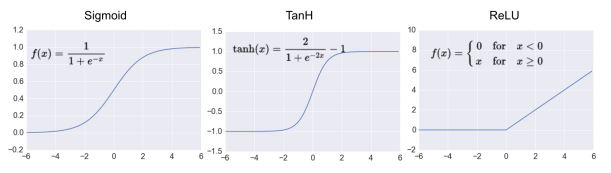
\includegraphics[width=0.8\linewidth,keepaspectratio]{kr4}
% \end{center}
% \end{frame}

% %%%%%%%%%%%%%%%%%%%%%%%%%%%%%%%%%%%%%%%%%%%%%%%%%%%
% \begin{frame}[fragile] \frametitle{Keras Losses}
% \begin{center}
% 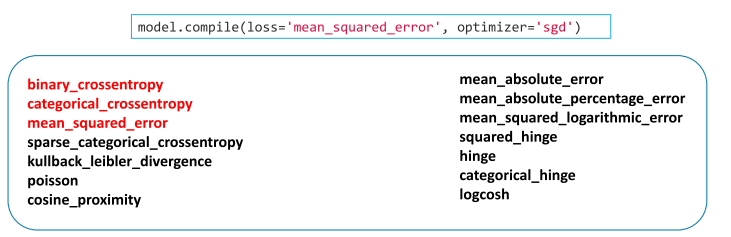
\includegraphics[width=\linewidth,keepaspectratio]{kr5}
% \end{center}
% \end{frame}

% %%%%%%%%%%%%%%%%%%%%%%%%%%%%%%%%%%%%%%%%%%%%%%%%%%%
% \begin{frame}[fragile] \frametitle{Keras Optimizers}
% An optimizer is one of the two arguments required for compiling a Keras model:

% \begin{lstlisting}
% from keras import optimizers 
% model = Sequential() 
% model.add(Dense(64, kernel_initializer='uniform', input_shape=(10,))) 
% model.add(Activation('tanh')) 
% sgd = optimizers.SGD(lr=0.01, decay=1e-6, momentum=0.9, nesterov=True) 
% model.compile(loss='mean_squared_error', optimizer=sgd)
% \end{lstlisting}
% \end{frame}

% %%%%%%%%%%%%%%%%%%%%%%%%%%%%%%%%%%%%%%%%%%%%%%%%%%%
% \begin{frame}[fragile] \frametitle{Keras Optimizers}

% \begin{itemize}
% \item  SGD :Stochastic gradient descent optimizer.
% \item RMSprop: RMSProp optimizer  is usually a good choice for recurrent neural networks.
% Adagrad
% \item Nadam : Much like Adam is essentially RMSprop with momentum, Nadam is Adam RMSprop with Nesterov
% momentum
% \item Adadelta
% \item Adam
% \item You can also use a wrapper class for native TensorFlow optimizers TFOptimizer
% \end{itemize}
% \end{frame}

% %%%%%%%%%%%%%%%%%%%%%%%%%%%%%%%%%%%%%%%%%%%%%%%%%%%
% \begin{frame}[fragile] \frametitle{Keras Optimizers}
% \begin{lstlisting}
% keras.optimizers.SGD(lr=0.01, momentum=0.0, decay=0.0, nesterov=False)
% keras.optimizers.RMSprop(lr=0.001, rho=0.9, epsilon=1e-08, decay=0.0) 
% keras.optimizers.Adagrad(lr=0.01, epsilon=1e-08, decay=0.0) 
% keras.optimizers.Adadelta(lr=1.0, rho=0.95, epsilon=1e-08, decay=0.0)
% keras.optimizers.Adam(lr=0.001, beta_1=0.9, beta_2=0.999, epsilon=1e-08, decay=0.0) 
% keras.optimizers.Nadam(lr=0.002, beta_1=0.9, beta_2=0.999, epsilon=1e-08, 
% schedule_decay=0.004) 

% keras.optimizers.TFOptimizer(optimizer) 
% \end{lstlisting}
% \end{frame}

% %%%%%%%%%%%%%%%%%%%%%%%%%%%%%%%%%%%%%%%%%%%%%%%%%%%
% \begin{frame}[fragile] \frametitle{ Learning Rate Scheduler}
% In Keras you have two types of learning rate schedule:
% \begin{center}
% 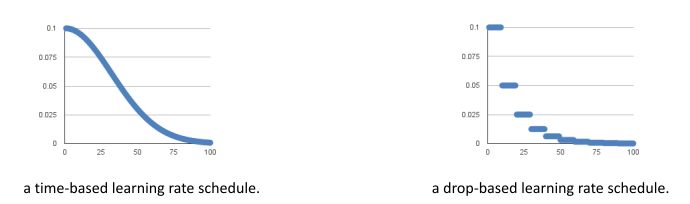
\includegraphics[width=\linewidth,keepaspectratio]{kr6}
% \end{center}
% \end{frame}

% %%%%%%%%%%%%%%%%%%%%%%%%%%%%%%%%%%%%%%%%%%%%%%%%%%%
% \begin{frame}[fragile] \frametitle{ Time based Learning Rate Scheduler}
% \begin{center}
% 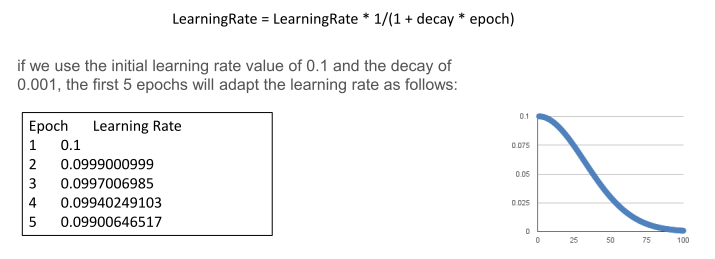
\includegraphics[width=\linewidth,keepaspectratio]{kr7}
% \end{center}
% \end{frame}

% %%%%%%%%%%%%%%%%%%%%%%%%%%%%%%%%%%%%%%%%%%%%%%%%%%%
% \begin{frame}[fragile] \frametitle{ Drop based Learning Rate Scheduler}
% \begin{center}
% 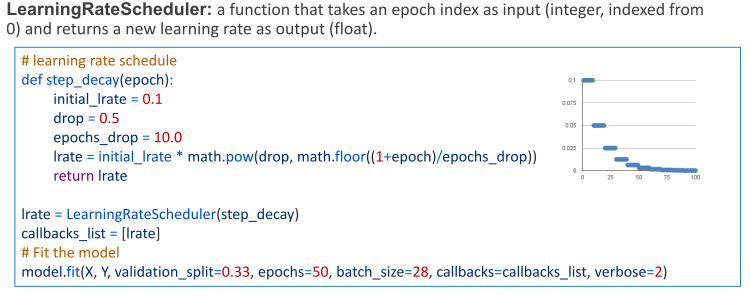
\includegraphics[width=\linewidth,keepaspectratio]{kr8}
% \end{center}
% \end{frame}


% %%%%%%%%%%%%%%%%%%%%%%%%%%%%%%%%%%%%%%%%%%%%%%%%%%%
% \begin{frame}[fragile] \frametitle{  Tips for Using Learning Rate}
% \begin{center}
% 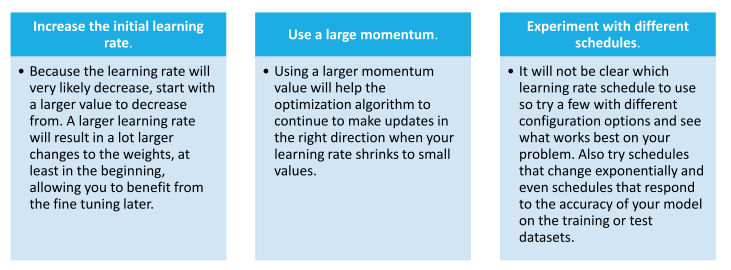
\includegraphics[width=\linewidth,keepaspectratio]{kr9}
% \end{center}
% \end{frame}

% %%%%%%%%%%%%%%%%%%%%%%%%%%%%%%%%%%%%%%%%%%%%%%%%%%%
% \begin{frame}[fragile] \frametitle{Keras Metrics}

% \begin{itemize}
% \item   Accuracy
% \begin{itemize}
% \item  binary\_accuracy
% \item  categorical\_accuracy
% \item  sparse\_categorical\_accuracy
% \item  top\_k\_categorical\_accuracy
% \item  sparse\_top\_k\_categorical\_accuracy
% \end{itemize}
% \item  Precision 
% \item  Recall
% \item  FScore
% \end{itemize}
% \begin{lstlisting}
% from keras import metrics 
% model.compile(loss='categorical_crossentropy', 
% optimizer='adadelta', 
% metrics=['accuracy', 'f1score', 'precision', 'recall'])
% \end{lstlisting}
% \end{frame}

% %%%%%%%%%%%%%%%%%%%%%%%%%%%%%%%%%%%%%%%%%%%%%%%%%%%
% \begin{frame}[fragile] \frametitle{Keras Metrics}
% Custom metrics can be passed at the compilation step. The function would need to 
% take (y\_true, y\_pred) as arguments and return a single tensor value.
% \begin{lstlisting}
% import keras.backend as K 
% def mean_pred(y_true, y_pred): 
% return K.mean(y_pred)
% model.compile(optimizer='rmsprop', loss='binary_crossentropy', 
% metrics=['accuracy', mean_pred])
% \end{lstlisting}
% \end{frame}


% %%%%%%%%%%%%%%%%%%%%%%%%%%%%%%%%%%%%%%%%%%%%%%%%%%%
% \begin{frame}[fragile] \frametitle{Keras Performance evaluation strategies}
% The large amount of data and the complexity of the models require very long training times.
% Keras provides a three convenient ways of evaluating your deep learning algorithms :
% \begin{itemize}
% \item Use an automatic verification dataset.
% \item Use a manual verification dataset.
% \item Use a manual k-Fold Cross Validation.
% \end{itemize}
% \end{frame}

% %%%%%%%%%%%%%%%%%%%%%%%%%%%%%%%%%%%%%%%%%%%%%%%%%%%
% \begin{frame}[fragile] \frametitle{Keras Performance evaluation strategies}
% \begin{center}
% 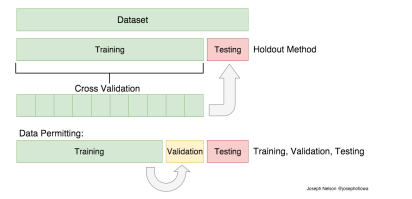
\includegraphics[width=\linewidth,keepaspectratio]{kr10}
% \end{center}
% \end{frame}

% %%%%%%%%%%%%%%%%%%%%%%%%%%%%%%%%%%%%%%%%%%%%%%%%%%%
% \begin{frame}[fragile] \frametitle{Automatic Verification Dataset}
% Keras can separate a portion of your training data into a validation dataset and evaluate the 
% performance of your model on that validation dataset each epoch
% \begin{center}
% 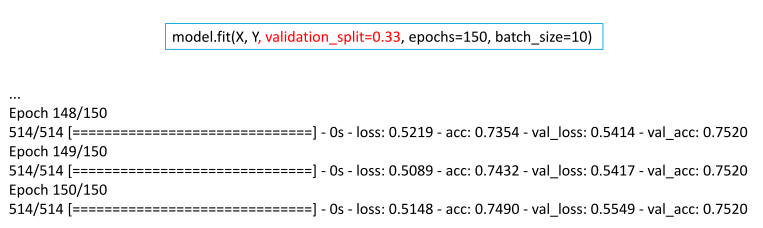
\includegraphics[width=\linewidth,keepaspectratio]{kr11}
% \end{center}
% \end{frame}

% %%%%%%%%%%%%%%%%%%%%%%%%%%%%%%%%%%%%%%%%%%%%%%%%%%%
% \begin{frame}[fragile] \frametitle{Manual Verification Dataset}
% Keras also allows you to manually specify the dataset to use for validation during training.
% \begin{lstlisting}
% # MLP with manual validation set
% from sklearn.model_selection import train_test_split
% import numpy
% # fix random seed for reproducibility
% seed = 7
% numpy.random.seed(seed)
% X_train, X_test, y_train, y_test = train_test_split(X, Y, test_size=0.33, random_state=seed)
% # Fit the model
% model.fit(X_train, y_train, validation_data=(X_test,y_test), epochs=150, batch_size=10)
% \end{lstlisting}
% \end{frame}

% %%%%%%%%%%%%%%%%%%%%%%%%%%%%%%%%%%%%%%%%%%%%%%%%%%%
% \begin{frame}[fragile] \frametitle{ Manual k-Fold Cross Validation}
% \begin{lstlisting}
% from sklearn.model_selection import StratifiedKFold
% kfold = StratifiedKFold(n_splits=10, shuffle=True, random_state=seed)
% cvscores = []
% for train, test in kfold.split(X, Y):
	% # create model
	% model = Sequential()
	% model.add(Dense(12, input_dim=8, activation='relu'))
	% model.add(Dense(8, activation='relu'))
	% model.add(Dense(1, activation='sigmoid'))
	% model.compile(loss='binary_crossentropy', optimizer='adam', metrics=['accuracy'])
	% # Fit the model
	% model.fit(X[train], Y[train], epochs=150, batch_size=10, verbose=0)
	% # evaluate the model
	% scores = model.evaluate(X[test], Y[test], verbose=0)
	% print("%s: %.2f%%" % (model.metrics_names[1], scores[1]*100))
	% cvscores.append(scores[1] * 100)
% print("%.2f%% (+/- %.2f%%)" % (numpy.mean(cvscores), numpy.std(cvscores)))
% \end{lstlisting}
% \end{frame}


% %%%%%%%%%%%%%%%%%%%%%%%%%%%%%%%%%%%%%%%%%%%%%%%%%%%
% \begin{frame}[fragile] \frametitle{Keras Regularizers}
% Nearly everything in Keras can be regularized to avoid overfitting 
% In addition to the Dropout layer, there are all sorts of other regularizers available, such as:
% \begin{itemize}
% \item  Weight regularizers
% \item  Bias regularizers
% \item  Activity regularizers
% \end{itemize}
% \begin{lstlisting}
% from keras import regularizers 
% model.add(Dense(64, input_dim=64, 
% kernel_regularizer=regularizers.l2(0.01), 
% activity_regularizer=regularizers.l1(0.01)))
% \end{lstlisting}
% \end{frame}

% %%%%%%%%%%%%%%%%%%%%%%%%%%%%%%%%%%%%%%%%%%%%%%%%%%%
% \begin{frame}[fragile] \frametitle{Keras Pickle}
% Saving/loading whole models (architecture + weights + optimizer state)
% \begin{lstlisting}
% from keras.models import load_model
% model.save('my_model.h5') # creates a HDF5 file 'my_model.h5'
% del model # deletes the existing model
% # returns a compiled model
% # identical to the previous one
% model = load_model('my_model.h5')
% \end{lstlisting}
% You can also save/load only a model's architecture or weights only. 
% \end{frame}

% %%%%%%%%%%%%%%%%%%%%%%%%%%%%%%%%%%%%%%%%%%%%%%%%%%%
% \begin{frame}[fragile] \frametitle{Keras Model Visualization}
% In case you want an image of your model :
% \begin{lstlisting}
% from keras.utils import plot_model
% plot_model(model, to_file='model.png')
% \end{lstlisting}
% \begin{center}
% 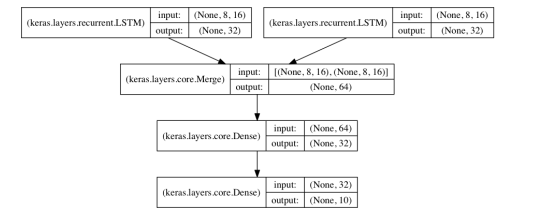
\includegraphics[width=\linewidth,keepaspectratio]{kr12}
% \end{center}
% \end{frame}


% %%%%%%%%%%%%%%%%%%%%%%%%%%%%%%%%%%%%%%%%%%%%%%%%%%%
% \begin{frame}[fragile] \frametitle{Keras Callbacks}
% Allow for function call during training:
% \begin{itemize}
% \item  Callbacks can be called at different points of training (batch or epoch) 
% \item  Existing callbacks: Early Stopping, weight saving after epoch 
% \item  Easy to build and implement, called in training function, fit()
% \end{itemize}
% \end{frame}

% %%%%%%%%%%%%%%%%%%%%%%%%%%%%%%%%%%%%%%%%%%%%%%%%%%%
% \begin{frame}[fragile] \frametitle{Keras Callbacks Examples}
% \begin{itemize}
% \item  TerminateOnNaN : Callback that terminates training when a NaN loss is encountered.
% \item  EarlyStopping: Stop training when a monitored quantity has stopped improving.
% \item  ModelCheckpoint : Save the model after every epoch.
% \begin{lstlisting}
% keras.callbacks.ModelCheckpoint(filepath, monitor='val_loss', verbose=0, 
% save_best_only=False, save_weights_only=False, mode='auto', period=1)
% \end{lstlisting}
% \item ReduceLROnPlateau: Reduce learning rate when a metric has stopped improving.
% \begin{lstlisting}
% keras.callbacks.ReduceLROnPlateau(monitor='val_loss', factor=0.1, 
% patience=10, verbose=0, mode='auto', epsilon=0.0001, cooldown=0, min_lr=0) 
% \end{lstlisting}
% \item Also, You can create a custom callback by extending the base class keras.callbacks.Callback
% \end{itemize}
% \end{frame}

% %%%%%%%%%%%%%%%%%%%%%%%%%%%%%%%%%%%%%%%%%%%%%%%%%%%
% \begin{frame}[fragile] \frametitle{Keras + TensorBoard: Visualizing Learning}
% \begin{itemize}
% \item  TensorBoard is a visualization tool provided with TensorFlow.
% \item  This callback writes a log for TensorBoard, which allows you to visualize dynamic graphs of 
% your training and test metrics, as well as activation histograms for the different layers in your 
% model.
% \begin{lstlisting}
% tbCallBack= keras.callbacks.TensorBoard(log_dir='./logs', 
% histogram_freq=0, batch_size=32, write_graph=True, 
% write_grads=False, write_images=False, embeddings_freq=0, 
% embeddings_layer_names=None, embeddings_metadata=None) 

% # Use your terminal
% tensorboard --logdir path_to_current_dir/logs
% \end{lstlisting}
% \end{itemize}
% \end{frame}


% %%%%%%%%%%%%%%%%%%%%%%%%%%%%%%%%%%%%%%%%%%%%%%%%%%%
% \begin{frame}
  % \begin{center}
    % {\Large Classification in Keras}
    
    % {Ref: Deep Learning A-Z - Udemy}
  % \end{center}
% \end{frame}


% %%%%%%%%%%%%%%%%%%%%%%%%%%%%%%%%%%%%%%%%%%%%%%%%%%%
% \begin{frame}[fragile] \frametitle{Customer Churn}
% Bank customers churn (exits)

% Dataset:
% \begin{center}
% 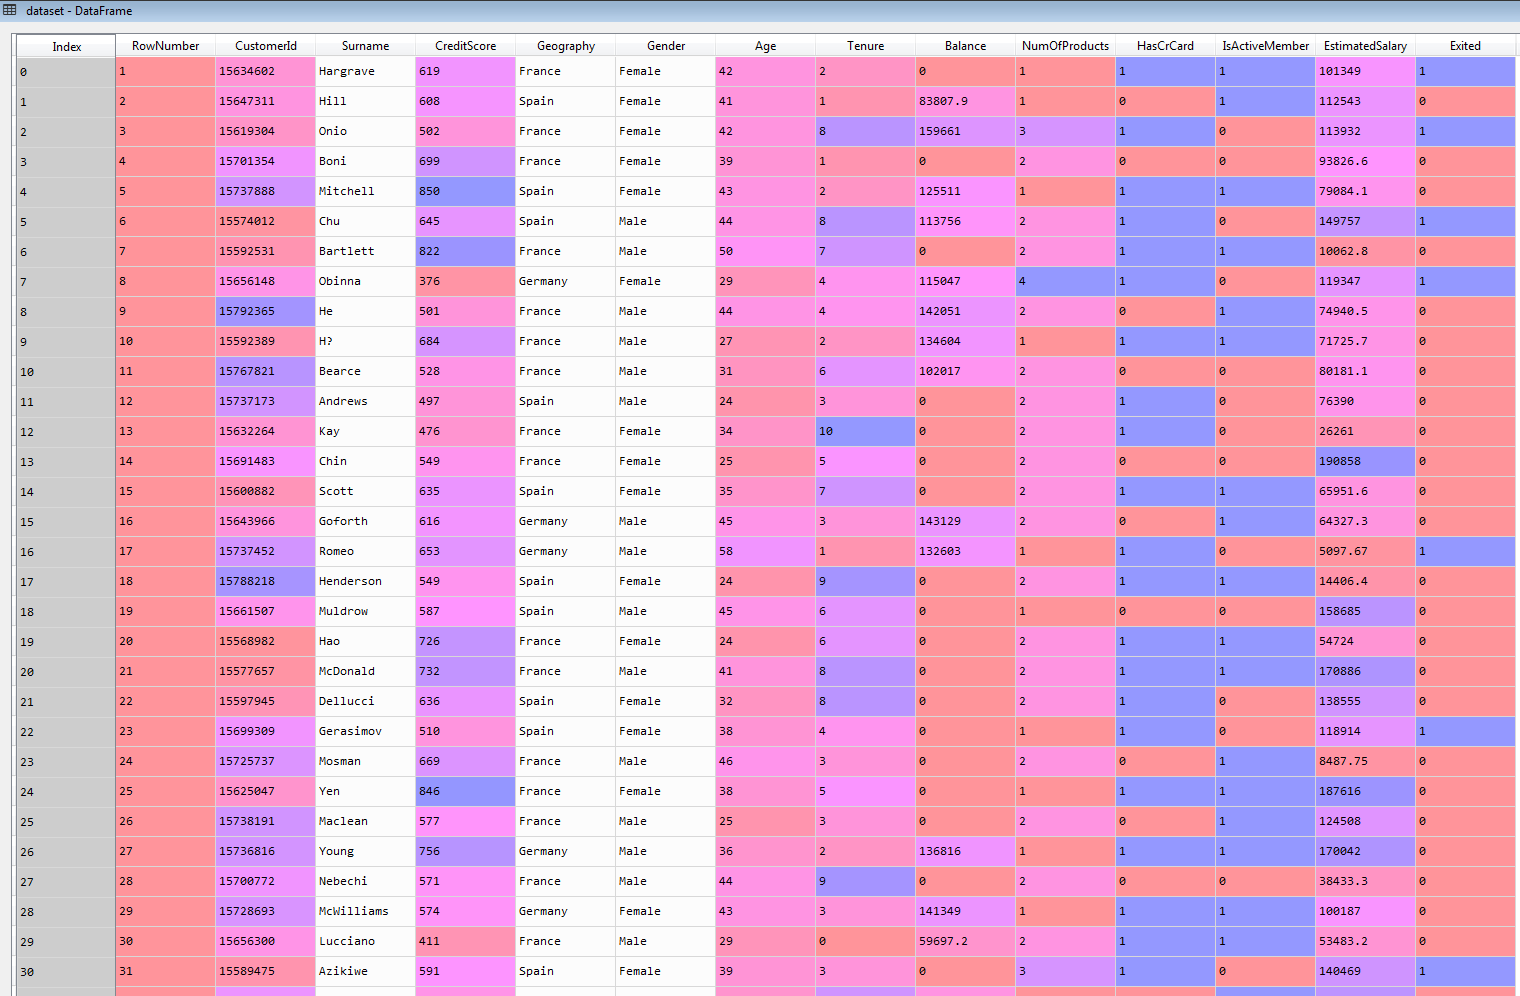
\includegraphics[width=0.7\linewidth,keepaspectratio]{kr13}
% \end{center}
% Target: ``Exited''.

% Inputs: Some of the other columns.
% \end{frame}

% %%%%%%%%%%%%%%%%%%%%%%%%%%%%%%%%%%%%%%%%%%%%%%%%%%%
% \begin{frame}[fragile] \frametitle{Get Inputs}
% \begin{lstlisting}
% # Importing the libraries
% import numpy as np
% import matplotlib.pyplot as plt
% import pandas as pd

% # Importing the dataset
% dataset = pd.read_csv('Churn_Modelling.csv')
% X = dataset.iloc[:, 3:13].values
% y = dataset.iloc[:, 13].values
% \end{lstlisting}
% First 2 columns are not relevant for modeling, so skipped.
% \end{frame}


% %%%%%%%%%%%%%%%%%%%%%%%%%%%%%%%%%%%%%%%%%%%%%%%%%%%
% \begin{frame}[fragile] \frametitle{Process Inputs}
% Convert categorical variables to Integers. 
% \begin{lstlisting}
% # Encoding categorical data
% from sklearn.preprocessing import LabelEncoder, OneHotEncoder
% labelencoder_X_1 = LabelEncoder()
% X[:, 1] = labelencoder_X_1.fit_transform(X[:, 1])
% labelencoder_X_2 = LabelEncoder()
% X[:, 2] = labelencoder_X_2.fit_transform(X[:, 2])
% # Country is not ordinal, so make it one hot
% onehotencoder = OneHotEncoder(categorical_features = [1])
% X = onehotencoder.fit_transform(X).toarray()
% X = X[:,1:]
% \end{lstlisting}
% Cities being non-ordinal (not ranked), need to be convrted to One-hot. So 3 new dummy columns got added.
% One of them is removed to avoid ``dummy variable trap'' ( multicollinear - a scenario in which two or more variables are highly correlated; in simple terms one variable can be predicted from the others.)
% \end{frame}

% %%%%%%%%%%%%%%%%%%%%%%%%%%%%%%%%%%%%%%%%%%%%%%%%%%%
% \begin{frame}[fragile] \frametitle{Process Inputs}
% Its necessary to normalize feature values
% \begin{lstlisting}
% # Feature Scaling
% from sklearn.preprocessing import StandardScaler
% sc = StandardScaler()
% X_train = sc.fit_transform(X_train)
% X_test = sc.transform(X_test)
% \end{lstlisting}
% Input X looks like:
% \begin{center}
% 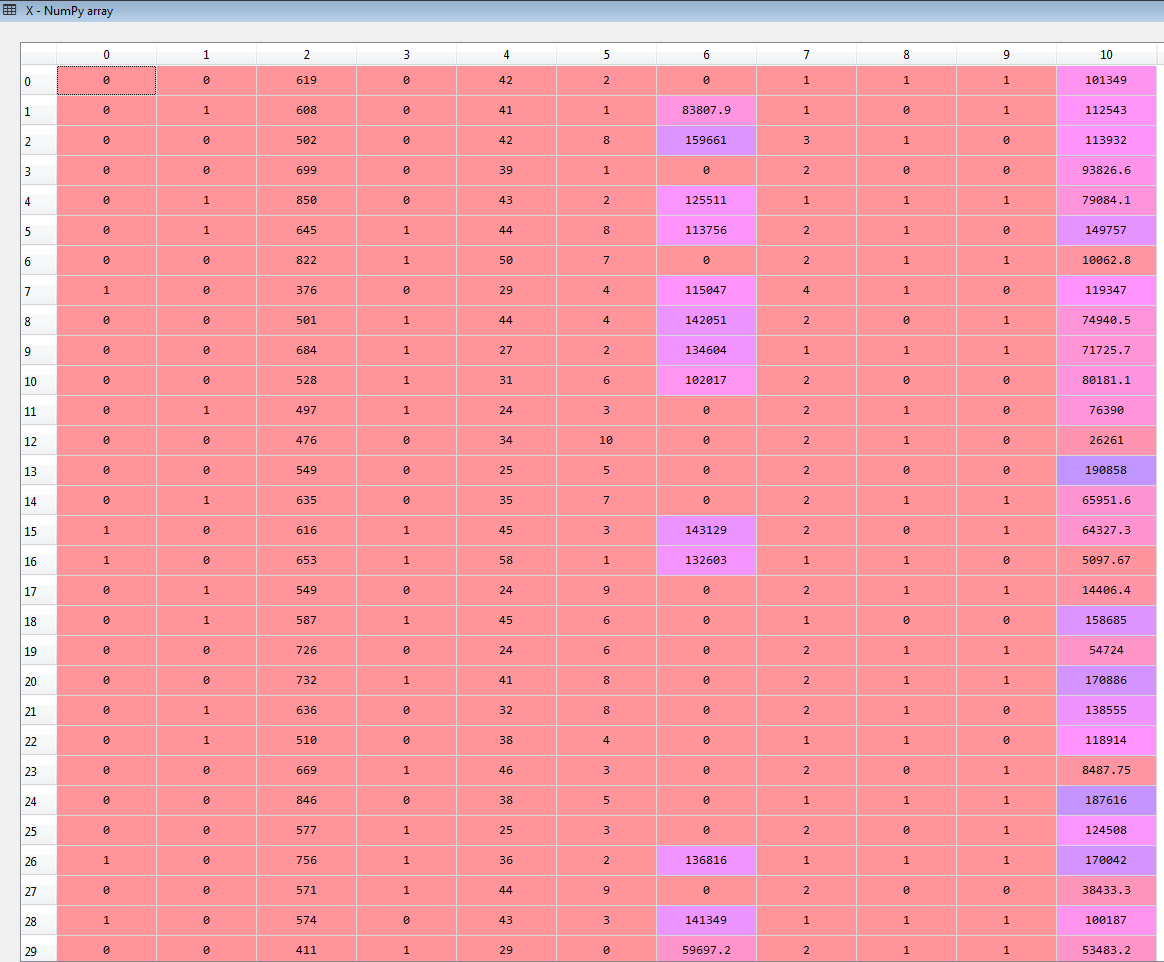
\includegraphics[width=0.4\linewidth,keepaspectratio]{kr14}
% \end{center}
% \end{frame}

% %%%%%%%%%%%%%%%%%%%%%%%%%%%%%%%%%%%%%%%%%%%%%%%%%%%
% \begin{frame}[fragile] \frametitle{Build Classifier}
% Basic NN, defined by layers one by one.
% \begin{lstlisting}
% import keras
% from keras.models import Sequential
% from keras.layers import Dense


% classifier = Sequential()
% classifier.add(Dense(6,kernel_initializer='uniform', activation='relu',input_shape=(11,)))
% \end{lstlisting}
% Adding Hidden layer and specifying input dimensions there. Dense is a function between two layers. It randomly inittializes the weights to small numbers close to 0 (but not 0).

% Tip: Number of nodes in the hidden layer = average of input and output dimensions. So, Avrg(11,1) = 6.
% \end{frame}

% %%%%%%%%%%%%%%%%%%%%%%%%%%%%%%%%%%%%%%%%%%%%%%%%%%%
% \begin{frame}[fragile] \frametitle{Build Classifier}
% Adding more layers
% \begin{lstlisting}
% classifier.add(Dense(6,kernel_initializer='uniform', activation='relu'))
% classifier.add(Dense(1,kernel_initializer='uniform', activation='sigmoid'))

% classifier.compile(optimzer='adam',loss="binary_crossentropy")
% \end{lstlisting}
% The last activation has to be sigmoid (or softamax for more than 2 categories) to get the probabilities.

% Finally compile by spcifying adam (a Stochastic Gradient Descent) algorithm. For more than 2 categories loss is ``categorical\_crossentropy''.
% \end{frame}


% %%%%%%%%%%%%%%%%%%%%%%%%%%%%%%%%%%%%%%%%%%%%%%%%%%%
% \begin{frame}[fragile] \frametitle{Fit with X and y}
% \begin{lstlisting}
% classifier.fit(X_train,y_train,batch_size=10, nb_epoch=100)

% Epoch 98/100
% 8000/8000 [==============================] - 1s 144us/step - loss: 0.4002 - acc: 0.8361
% Epoch 99/100
% 8000/8000 [==============================] - 1s 143us/step - loss: 0.4001 - acc: 0.8344
% Epoch 100/100
% 8000/8000 [==============================] - 1s 131us/step - loss: 0.4004 - acc: 0.8339
% \end{lstlisting}
% Batch is the number of records after which the weights are updated.
% Accuracy goes on increasing and reaches to 83\%
% \end{frame}



% %%%%%%%%%%%%%%%%%%%%%%%%%%%%%%%%%%%%%%%%%%%%%%%%%%%
% \begin{frame}[fragile] \frametitle{Using model}
% \begin{lstlisting}
% # Predicting the Test set results
% y_pred = classifier.predict(X_test)
% y_pred = (y_pred > 0.5)

% # Making the Confusion Matrix
% from sklearn.metrics import confusion_matrix
% cm = confusion_matrix(y_test, y_pred)

% array([[1542,   53],
       % [ 261,  144]], dtype=int64)
% \end{lstlisting}
% Need to decide THRESHOLD to decide boolean output. 0.50 is ok here.
% \end{frame}

% %%%%%%%%%%%%%%%%%%%%%%%%%%%%%%%%%%%%%%%%%%%%%%%%%%%
% \begin{frame}[fragile] \frametitle{Predict}
% Unseen Customer \ldots
% \begin{itemize}
% \item Geography: France
% \item Credit Score: 600
% \item Gender: Male
% \item Age: 40 years old
% \item Tenure: 3 years
% \item Balance: \$60000
% \item Number of Products: 2
% \item Does this customer have a credit card ? Yes
% \item Is this customer an Active Member: Yes
% \item Estimated Salary: \$50000
% \end{itemize}
% Will the customer leave?
% \end{frame}

% %%%%%%%%%%%%%%%%%%%%%%%%%%%%%%%%%%%%%%%%%%%%%%%%%%%
% \begin{frame}[fragile] \frametitle{Predict}
% \begin{lstlisting}
% new_test_x = np.array([[0,0,600,1,40,3,60000, 2,1,1,50000]])
% new_test_x = sc.transform(new_test_x)
% new_prediction = classifier.predict(new_test_x)
% new_prediction = (new_prediction > 0.5)
% \end{lstlisting}
% FALSE!!!
% \end{frame}

% %%%%%%%%%%%%%%%%%%%%%%%%%%%%%%%%%%%%%%%%%%%%%%%%%%%
% \begin{frame}[fragile] \frametitle{Evaluating}
% \begin{itemize}
% \item Using only one x\_test set may not give a representative result and accuracy. 
% \item Need to use K-fold which uses different test sets for evaluation. 
% \item This solves High Variance problems (diff test sets given divergent results).
% \item For k=10 folds, we will get 10 accuracies. 
% \item We can find mean and std deviation of those 10 values. 
% \item Based on these, we can be one of following 4 cases
% \end{itemize}
% \begin{center}
% 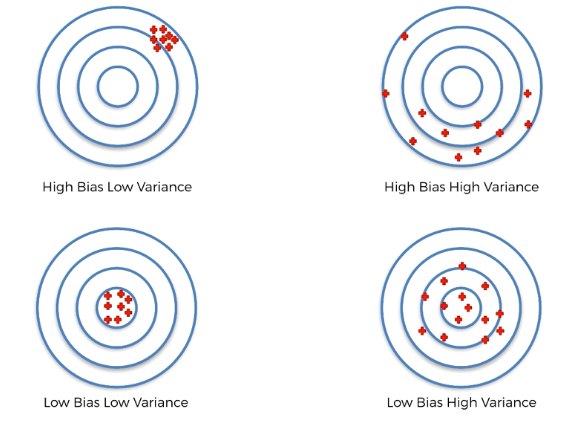
\includegraphics[width=0.35\linewidth,keepaspectratio]{kr15}
% \end{center}

% \end{frame}

% %%%%%%%%%%%%%%%%%%%%%%%%%%%%%%%%%%%%%%%%%%%%%%%%%%%
% \begin{frame}[fragile] \frametitle{K-Fold with Keras}
% \begin{itemize}
% \item K-fold functionality is in Scikit Learn.
% \item Keras can use it by wrapping it.
% \item KerasClassifier needs a function that builds and returns classifier NN
% \end{itemize}
% \begin{lstlisting}
% from keras.wrappers.scikit_learn import KerasClassifier
% from sklearn.model_selection import cross_val_score

% def build_classifier():
    % classifier = Sequential()
    % classifier.add(Dense(6,kernel_initializer='uniform', activation='relu',input_shape=(11,)))
    % classifier.add(Dense(6,kernel_initializer='uniform', activation='relu'))
    % classifier.add(Dense(1,kernel_initializer='uniform', activation='sigmoid'))
    % classifier.compile(optimizer='adam',loss="binary_crossentropy", metrics = ['accuracy'])
    % return classifier
% \end{lstlisting}
% \end{frame}

% %%%%%%%%%%%%%%%%%%%%%%%%%%%%%%%%%%%%%%%%%%%%%%%%%%%
% \begin{frame}[fragile] \frametitle{K-Fold with Keras}
% \begin{itemize}
% \item Individual classifiers within the function will be spawed on different test-train sets, during K-folds
% \item A common classfier representing total classification process is defined with the build\_classifier function.
% \item cross\_val\_score from sklearn will return set of all accuracies.
% \item Find mean and std dev to see where we are.
% \end{itemize}
% \begin{lstlisting}
% classifier_common = KerasClassifier(build_fn=build_classifier,batch_size = 10, nb_epoch=100)
% accuracies = cross_val_score(estimator=classifier_common,X=X_train,y=y_train,cv=10,n_jobs=-1)
% mean = accuracies.mean()
% variance = accuracies.std()
% \end{lstlisting}
% Put -1 for n\_jobs to use all CPUs.
% \end{frame}

